\documentclass[conference]{IEEEtran}

\usepackage{amsmath, amsthm, amssymb}
\usepackage{latexsym}
\usepackage{graphicx}
\usepackage{verbatim}
\usepackage{mathrsfs}
\usepackage{float}
\usepackage[lofdepth, lotdepth]{subfig}
\usepackage{array}
\usepackage{url}
\usepackage{algorithm}
\usepackage[noend]{algorithmic}
\usepackage{cite}
%\usepackage[table]{xcolor}
\usepackage[dvipsnames]{xcolor}
\usepackage{enumerate}
\usepackage{eucal}
\usepackage{stmaryrd}
\usepackage{mathtools}
\usepackage{pgf}
\usepackage{tikz}
\usetikzlibrary{arrows,automata}
\usepackage[latin1]{inputenc}
%\usepackage{tikz}
\usetikzlibrary{automata,positioning}
%\usepackage{natbib}
%\usepackage{geometry}
%\geometry{legalpaper, landscape, margin=1in}
%\addtolength{\topmargin}{8mm}
%\addtolength{\topmargin}{0.43in}



%\usepackage[top=0.6in, bottom=0.6in, left=0.6in, right=0.61in]{geometry}
%\usepackage[margin=1in]{geometry}
\usepackage{mathtools}
\DeclarePairedDelimiter\ceil{\lceil}{\rceil}
\DeclarePairedDelimiter\floor{\lfloor}{\rfloor}

%\usepackage{algpseudocode}
%\floatname{algorithm}{Procedure}
\renewcommand{\algorithmicrequire}{\textbf{Input:}}
\renewcommand{\algorithmicensure}{\textbf{Output:}}

% Generated with LaTeXDraw 2.0.8
% Mon May 09 15:51:58 SGT 2011
%\usepackage[usenames,dvipsnames]{pstricks}
%\usepackage[crop=off]{auto-pst-pdf}
%\usepackage{epsfig}
%\usepackage{pst-grad} % For gradients
%\usepackage{pst-plot} % For axes

\theoremstyle{plain}
\newtheorem{theorem}{Theorem}
\newtheorem{proposition}{Proposition}
\newtheorem{lemma}{Lemma}
\newtheorem{conjecture}{Conjecture}
\newtheorem{corollary}{Corollary}
%\newtheorem{algorithm}{Algorithm}
\newtheorem{construction}{Construction}
\theoremstyle{definition}
\newtheorem{definition}{Definition}
\newtheorem{example}{Example}
\newtheorem{remark}{Remark}


\newcommand{\hm}[1]{{\color{magenta}(HM: #1)}}


%%%%%%%%%%%%%%%%%%%%%%%%%%%%%%%%%%%%%%%%%%%%%%%%%%%%%
%\mathcal{}

\newcommand{\A}{{\mathcal A}}
\newcommand{\B}{{\mathcal B}}
\newcommand{\C}{{\mathcal C}}
\newcommand{\D}{{\mathcal D}}
\newcommand{\cE}{{\mathcal E}}
\newcommand{\F}{{\mathcal F}}
\newcommand{\G}{{\mathcal G}}
\newcommand{\cH}{{\mathcal H}}
\newcommand{\I}{{\mathcal I}}
\newcommand{\J}{{\mathcal J}}
\newcommand{\K}{{\mathcal K}}
\newcommand{\cL}{{\mathcal L}}
\newcommand{\Q}{{\mathcal Q}}
\newcommand{\X}{{\mathcal X}}
\newcommand{\Z}{{\mathcal Z}}
\newcommand{\W}{{\mathcal W}}

\newcommand{\Y}{{\mathcal Y}}
\newcommand{\V}{{\mathcal V}}
\newcommand{\R}{{\mathcal R}}
\newcommand{\N}{{\mathcal N}}
\newcommand{\cS}{{\mathcal S}}

%\mathcal{}
%%%%%%%%%%%%%%%%%%%%%%%%%%%%%%%%%%%%%%%%%%%%%%%%%%%%%


%%%%%%%%%%%%%%%%%%%%%%%%%%%%%%%%%%%%%%%%%%%%%%%%%%%%%
%\mathbfsl{}

\DeclareMathAlphabet{\mathbfsl}{OT1}{ppl}{b}{it} %{OT1}{cmr}{bx}{it}

\newcommand{\bM}{{\mathbfsl{M}}}
\newcommand{\bN}{{\mathbfsl{N}}}
\newcommand{\bI}{{\mathbfsl I}}
\newcommand{\bJ}{{\mathbfsl J}}
\newcommand{\bP}{{\mathbfsl P}}
\newcommand{\bQ}{{\mathbfsl Q}}
\newcommand{\bF}{{\mathbfsl F}}
\newcommand{\bH}{{\mathbfsl H}}

\newcommand{\bL}{\mathbfsl{L}}
\newcommand{\bA}{{\mathbfsl A}}
\newcommand{\bB}{{\mathbfsl B}}
\newcommand{\bC}{{\mathbfsl C}}
\newcommand{\bE}{{\mathbfsl E}}
\newcommand{\bX}{\mathbfsl{X}}
\newcommand{\bY}{\mathbfsl{Y}}
\newcommand{\bU}{\mathbfsl{U}}

\newcommand{\ba}{{\mathbfsl a}}
\newcommand{\bb}{{\mathbfsl b}}
\newcommand{\bp}{{\mathbfsl p}}
\newcommand{\bq}{{\mathbfsl q}}

\newcommand{\bu}{{\mathbfsl u}}
\newcommand{\bv}{{\mathbfsl v}}
\newcommand{\bff}{{\mathbfsl f}}
\newcommand{\bs}{{\mathbfsl s}}
\newcommand{\by}{{\mathbfsl y}}

\newcommand{\bd}{{\mathbfsl{d}}}
\newcommand{\bk}{{\mathbfsl{k}}}

\newcommand{\bc}{{\mathbfsl c}}
\newcommand{\bO}{{\mathbfsl 0}}
\newcommand{\bw}{{\mathbfsl{w}}}
\newcommand{\bg}{{\mathbfsl{g}}}
\newcommand{\br}{{\mathbfsl{r}}}
\newcommand{\bx}{{\mathbfsl{x}}}
\newcommand{\bz}{{\mathbfsl{z}}}
\newcommand{\bZ}{\mathbfsl{Z}}
\newcommand{\bG}{{\mathbfsl{G}}}
\newcommand{\be}{{\mathbfsl e}}
\newcommand{\bl}{{\mathbfsl l}}
\newcommand{\bbt}{\boldsymbol{\beta}}
\newcommand{\bsg}{{\boldsymbol{\sigma}}}

%\mathbfsl
%%%%%%%%%%%%%%%%%%%%%%%%%%%%%%%%%%%%%%%%%

%%%%%%%%%%%%%%%%%%%%%%%%%%%%%%%%%%%%%%%%%%%%%%%%%%%%%%%%
%\mathbb

\newcommand{\bbE}{{\mathbb E}}
\newcommand{\bbF}{{\mathbb F}}
\newcommand{\bbN}{{\mathbb N}}
\newcommand{\bbP}{{\mathbb P}}
\newcommand{\bbZ}{{\mathbb Z}}
\newcommand{\bbR}{{\mathbb R}}
\newcommand{\ff}{\mathbb{F}}
\newcommand{\ft}{\mathbb{F}_2}
\newcommand{\fq}{\mathbb{F}_q}
\newcommand{\fqn}{\mathbb{F}_q^n}

%\mathbb
%%%%%%%%%%%%%%%%%%%%%%%%%%%%%%%%%%%%%%%%%%%%%%%%%%%%%%%%

%%%%%%%%%%%%%%%%%%%%%%%%%%%%%%%%%%%%%%%%%%%%%%%%%%%%%%%
%\mathfrak

\newcommand{\fkD}{{\mathfrak D}}
\newcommand{\fkE}{{\mathfrak E}}
\newcommand{\fkJ}{{\mathfrak J}}
\newcommand{\fkC}{{\mathfrak C}}
\newcommand{\vu}{{\sf u}}
\newcommand{\vv}{{\sf v}}
%\mathfrak
%%%%%%%%%%%%%%%%%%%%%%%%%%%%%%%%%%%%%%%%%%%%%%%%%%%%%%%


%%%%%%%%%%%%%%%%%%%%%%%%%%%%%%%%%%%%%%%%%%%%%%%%%%%%%%%%
%Arrows
\newcommand{\lra}{\longrightarrow}
\newcommand{\Lra}{\Longrightarrow}
\newcommand{\Llra}{\Longleftrightarrow}
\newcommand{\nto}{\nrightarrow}
\newcommand{\ra}{\rightarrow}

%Arrows
%%%%%%%%%%%%%%%%%%%%%%%%%%%%%%%%%%%%%%%%%%%%%%%%%%%%%%%%

%%%%%%%%%%%%%%%%%%%%%%%%%%%%%%%%%%%%%%%%%%%%%%%%%%%%%%%%
%Greek characters
\newcommand{\al}{\alpha}
\newcommand{\bt}{\beta}
\newcommand{\vep}{\varepsilon}
\newcommand{\de}{\delta}
\newcommand{\ph}{\varphi}
\newcommand{\om}{\omega}
\newcommand{\kp}{\kappa}
\newcommand{\kpq}{\kappa_q}
\newcommand{\mn}{\mathbfsl N}
\newcommand{\De}{\Delta}
\newcommand{\deo}{{\delta}_0}
\newcommand{\epo}{{\varepsilon}_0}
\newcommand{\ga}{\gamma}
\newcommand{\Ga}{\Gamma}
\newcommand{\Gnr}{\Gamma(n,\rho)}
\newcommand{\lam}{\lambda}
\newcommand{\si}{\sigma}

%Greek characters
%%%%%%%%%%%%%%%%%%%%%%%%%%%%%%%%%%%%%%%%%%%%%%%%%%%%%%%%

%%%%%%%%%%%%%%%%%%%%%%%%%%%%%%%%%%%%%%%%%%%%%%%%%%%%%%%%
%Miscellaneous

\newcommand{\entropy}{{\sf H}}
\newcommand{\en}{{\sf H}}
\newcommand{\ent}{{\sf H}_2}
\newcommand{\mutualinfo}{{\sf I}}
\newcommand{\mi}{{\sf I}}
\newcommand{\supp}{{\sf supp}}
\newcommand{\dist}{{\mathsf{d}}}
\newcommand{\weight}{{\mathsf{wt}}}
\newcommand{\spn}{{\mathsf{span}_q}}

\newcommand{\ppmod}[1]{~({\rm mod~}#1)}

\newcommand{\rank}{{\mathsf{rank}_q}}
\newcommand{\rankt}{{\mathsf{rank}_2}}

%%%%%%%%%%%%%%%%%%%%%%%%%%%%%%%%%%%%%%%%%%%%%%%%%%%%%
%\mathscr
%\newcommand{\cC}{{\mathscr{C}}}
%\newcommand{\cG}{{\mathscr{G}}}
%\newcommand{\cV}{{\mathscr{V}}}
%\newcommand{\cE}{{\mathscr{E}}}
%\newcommand{\cH}{{\mathscr{H}}}
%\mathscr
%%%%%%%%%%%%%%%%%%%%%%%%%%%%%%%%%%%%%%%%%%%%%%%%%%%%%


\newcommand{\define}{\stackrel{\mbox{\tiny $\triangle$}}{=}}

\newcommand{\btd}{\bigtriangledown}

\newcommand{\ct}{\centerline}
\newcommand{\nin}{\noindent}
\newcommand{\ind}{\indent}

\newcommand{\seq}{\subseteqeq}


\renewcommand{\ge}{\geqslant}
\renewcommand{\le}{\leqslant}
\newcommand{\lek}{{{\le}k}}

\newcommand{\rate}{{\rm rate}}
\newcommand{\Irr}{{\rm Irr}}

\newcommand{\et}{{\emph{et al.}}}

\newcommand{\vM}{{{\sf var}}(\mathbfsl{M})}
\newcommand{\gM}{{{\sf gr}}(\mathbfsl{M})}
\newcommand{\sG}{{{\sf supp}}(\mathbfsl{G})}

\newcommand{\jmax}{j_{\max}}
\newcommand{\jmin}{j_{\min}}

\newcommand{\bMi}{\mathbfsl{M}^{(i)}}
\newcommand{\bMip}{\mathbfsl{M}^{(i')}}
\newcommand{\bMo}{\mathbfsl{M}^{(1)}}
\newcommand{\bMt}{\mathbfsl{M}^{(2)}}
\newcommand{\Ri}{R^{(i)}}
\newcommand{\Rip}{R^{(i')}}
\newcommand{\Ro}{R^{(1)}}
\newcommand{\Rt}{R^{(2)}}

\newcommand{\su}{{\sf u}}
\newcommand{\sv}{{\sf v}}
\newcommand{\sw}{{\sf w}}

\newcommand{\tA}{\mathtt{A}}
\newcommand{\tT}{\mathtt{T}}
\newcommand{\tC}{\mathtt{C}}
\newcommand{\tG}{\mathtt{G}}
\newcommand{\GC}{$\mathtt{GC}$}

\newcommand{\enc}{\textsc{Enc}}
\newcommand{\dec}{\textsc{Dec}}
\newcommand{\indexenc}{\textsc{IndexEnc}}


\newcommand{\Lburst}{{\rm L}^{\rm burst}}
\newcommand{\Dindel}{{\cal D}^{\rm indel}}
\newcommand{\Bindel}{{\cal B}^{\rm indel}}
\newcommand{\Bedit}{{\cal B}^{\rm edit}}
\newcommand{\Bburst}{{\cal B}^{\rm burst}}

%Miscellaneous
%%%%%%%%%%%%%%%%%%%%%%%%%%%%%%%%%%%%%%%%%%%%%%%%%%%%%%%%

\renewcommand{\qedsymbol}{$\blacksquare$}


\IEEEoverridecommandlockouts
\begin{document}

\pagestyle{empty}

%\title{An Efficient Solution Combining Error Correction and Constrained Codes for DNA-Based Data Storage\\[-5mm]}
%\title{An Efficient Combination of Error Correction Codes and Constrained Codes for DNA-Based Data Storage\\[-5mm]}
\title{On the Design of Codes for DNA Computing: Secondary Structure Avoidance Codes\\[-3mm]}

%\title{Coding for Runlength Limited and \GC-content Constraint with Error-Correction for DNA-Based Data Storage\\[-4mm]}
%\title{Linear-time Encoder for Error-Control Codes \\for DNA-Based Data Storage\\[-4mm]}
%\author{\IEEEauthorblockN{Tuan Thanh Nguyen\IEEEauthorrefmark{1},
%Kui Cai\IEEEauthorrefmark{1}, 
%Han Mao Kiah\IEEEauthorrefmark{2},
%and Kees A. Schouhamer Immink\IEEEauthorrefmark{3}}\\[-3mm]
%\IEEEauthorblockA{
%\IEEEauthorrefmark{1}
%Science, Mathematics and Technology Cluster, Singapore University of Technology and Design, Singapore 487372\\
%\IEEEauthorrefmark{2}%
%School of Physical and Mathematical Sciences, Nanyang Technological University, Singapore 637371\\
%\IEEEauthorrefmark{3}%
%Turing Machines Inc, Willemskade 15d, 3016 DK Rotterdam, The Netherlands\\
%Emails: \{tuanthanh\_nguyen, cai\_kui\}@sutd.edu.sg, hmkiah@ntu.edu.sg, immink@turing-machines.com\\[-4mm]
%}
%}

\author{\IEEEauthorblockN{Tuan Thanh Nguyen\IEEEauthorrefmark{1},
Kui Cai\IEEEauthorrefmark{1},
Han Mao Kiah\IEEEauthorrefmark{2},
Duc Tu Dao\IEEEauthorrefmark{2},  
and Kees A. Schouhamer Immink\IEEEauthorrefmark{3}}\\[-3mm]
\IEEEauthorblockA{
\IEEEauthorrefmark{1}
Science, Mathematics and Technology Cluster, Singapore University of Technology and Design, Singapore 487372\\
\IEEEauthorrefmark{2}%
School of Physical and Mathematical Sciences, Nanyang Technological University, Singapore 637371\\
\IEEEauthorrefmark{3}%
Turing Machines Inc, Willemskade 15d, 3016 DK Rotterdam, The Netherlands\\
Emails: \{tuanthanh\_nguyen, cai\_kui\}@sutd.edu.sg, \{hmkiah,daoductu001\}@ntu.edu.sg, immink@turing-machines.com\\[-4mm]
}
}
\maketitle
\begin{comment}
\author{%
  \IEEEauthorblockN{Anonymous Authors}
  %\IEEEauthorblockA{%
    %Please do NOT provide authors' names and affiliations\\
    %in the paper submitted for review, but keep this placeholder.\\
    %ISIT23 follows a \textbf{double-blind reviewing policy}.}
}
\end{comment}
\maketitle
\begin{comment}
\author{\IEEEauthorblockN{Tuan Thanh Nguyen\IEEEauthorrefmark{1},
Kui Cai\IEEEauthorrefmark{1},
and {\color{blue}{Kees A. Schouhamer Immink}}\IEEEauthorrefmark{2}}\\[-3mm]
%and Han Mao Kiah\IEEEauthorrefmark{3}}\\[-3mm]
\IEEEauthorblockA{
\IEEEauthorrefmark{1}%
Singapore University of Technology and Design, Singapore 487372\\
\IEEEauthorrefmark{2}%
Turing Machines Inc, Willemskade 15d, 3016 DK Rotterdam, The Netherlands\\
%\IEEEauthorrefmark{3}%
%School of Physical and Mathematical Sciences, Nanyang Technological University, Singapore 637371  hmkiah@ntu.edu.sg\\
Emails: \{tuanthanh\_nguyen, cai\_kui\}@sutd.edu.sg, immink@turing-machines.com\\[-4mm]
}
}
\maketitle
\end{comment}



%SECTION ABSTRACT
\hspace{-3mm}\begin{abstract}

In this work, we investigate a challenging problem, which has been considered to be an important criterion in designing codewords for DNA computing purposes, namely {\em secondary structure avoidance} in single-stranded DNA molecules. In short, secondary structure refers to the tendency of a single-stranded DNA sequence to fold back upon itself, thus becoming inactive in the computation process. 
While some design criteria that reduces the possibility of secondary structure formation has been proposed by Milenkovic and Kashyap (2006), the main contribution of this work is to provide an explicit construction of DNA codes that completely avoid secondary structure of arbitrary stem length.

Formally, given codeword length $n$ and arbitrary integer $m\ge 2$, we provide efficient methods to construct DNA codes of length $n$ that avoid secondary structure of any stem length more than or equal to $m$. Particularly, when $m=3$, our constructions yield a family of DNA codes of rate 1.3031 bits/nt, while the highest rate found in the prior art was 1.1609 bits/nt. In addition, for $m\ge 3\log n + 4$, we provide an efficient encoder that incurs only one redundant symbol.

%In addition, for sufficiently large $m=\Theta(\log n)$, we show that there exist codes with at most one redundant symbol. 
%Therefore, the design of secondary structure avoidance codes is crucial for DNA computing purposes. 
%the most important criterion in designing codewords for DNA computing purposes is that the codewords should not form secondary structures that cause them to become computationally inactive
%DNA sequences with secondary structures are less active chemically and are needed to unfold before reading. Formation of Secondary Structure

%We primarily focus on design considerations pertaining to the phenomena of secondary structure formation in single-stranded DNA molecules and non-selective cross-hybridization. Secondary structure formation refers to the tendency of single-stranded DNA sequences to fold back upon themselves, thus becoming inactive in the computation process

\end{abstract}
% section INTRODUCTION

\section{Introduction}
DNA computing is an emerging branch of computing that uses DNA, biochemistry, and molecular biology hardware. 
The field of DNA computation started with the following demonstration by Adleman in 1994~\cite{adle:1994}. In this seminal experiment, Adleman solved an instance of the directed traveling salesperson problem by first representing each city with a synthetic DNA molecule. Then by allowing the strands to hybridize in a highly parallel fashion, Adleman obtained the desired solution. Since then, similar methods have been expanded to several attractive applications, including the development of storage technologies \cite{church2012,fountain2017,Organick:2018,goldman2013}, and cell-based computation systems for cancer diagnostics and treatment \cite{son:2004}. Recently, the hybridization process was exploited to allow random access in DNA data storage~\cite{yazdi:2017}.
%The field of DNA computing started with the demonstration of a computing application by Adleman in 1994 \cite{adle:1994} when he managed to solve a specific instance of the directed travelling salesman problem by using DNA molecules where each one of them represents a city that had to be visited. Since then, it has been expanded to several attractive applications, particularly including the development of storage technologies \cite{church2012,fountain2017,Organick:2018,goldman2013}, and cell-based computation systems for cancer diagnostics and treatment \cite{son:2004}.

%synthetic controllers and reaction networks \cite{Ku:2018}
In DNA computing, only short single-stranded DNA sequences (or {\em oligonucleotide sequences}) are used, where each of them is an oriented word consisting of four bases (or {\em nucleotides}): Adenine ({\bf A}), Thymine  ({\bf T}), Cytosine ({\bf C}), and Guanine ({\bf G}). A set of encoded DNA sequences (also called DNA codewords), that satisfies certain special properties (or {\em constraints}) for DNA computing purposes, is called a DNA code. A broad description of the kinds of constraint problems that arise in coding for DNA computing was introduced by Milenkovic and Kashyap in 2006 \cite{O2:2005}, including {\em constant {\bf G}{\bf C}-content constraint} (refers to the percentage of nucleotides that are either {\bf G} or {\bf C}), {\em Hamming distance constraint} (that requires DNA codewords to be sufficiently different among themselves), and {\em secondary structure formation avoidance constraint} (that prevents DNA sequence to fold back upon itself, and consequently becoming inactive in the computation process). 
Similar considerations were described in~\cite{yazdi:2018, chee:2020} for the design of primer address sequences in random access of DNA-based data storage systems.
While constant {\bf G}{\bf C}-content constraint and Hamming distance constraint have been extensively investigated \cite{K:2021, KDG:2021, O:2005, O2:2005, TT:2021, KING:2003, KING:2005, segmented}, the study for secondary structure avoidance is much less profound. 


%Since then, the design of DNA constrained codes has been extensively investigated \cite{K:2021, KDG:2021, O:2005, O2:2005, TT:2021, KING:2003, KING:2005, cai2019}, including the study of: {\em constant {\bf G}{\bf C}-content constraint} (refers to the percentage of nucleotides that are either {\bf G} or {\bf C}, see, for example, \cite{cai2019, TT:2021}),  runlength-limited constraint (refers to the restriction on the repetition of identical nucleotides, see \cite{K:2021,cai2019}), {\em Hamming distance constraint, reverse-complement constraint} (that require DNA codewords are sufficiently different among themselves, their reverse sequences, and their reverse-complement sequences, see \cite{K:2021, KDG:2021}, and probably the most important constraint, as emphasised in \cite{O:2005,O2:2005,Bres:1986}, is the {\em secondary structure formation avoidance constraint}, which is also the main focus of this work. 

For a DNA sequence, a secondary structure is formed by a chemically active to fold back onto itself by complementary base pair hybridization (illustrated via Figure 1). Here, the {\em Watson-Crick complement} is defined as: $\overline{{\bf A}}={\bf T}, \overline{\bf T}={\bf A}, \overline{\bf C}={\bf G}$, and $\overline{\bf G}={\bf C}$. For a sequence $\bx=x_1x_2x_3\ldots x_{n-1}x_n$ over the DNA alphabet $\D=\{{\bf A}, {\bf T}, {\bf C}, {\bf G}\}$, the {\em reverse-complement} of $\bx$ is defined as ${\rm RC}({\bx})={\overline{x_n}} \text{ } \overline{x_{n-1}}\ldots  \overline{x_3}  \text{ } \overline{x_2}  \text{ } \overline{x_1}$. In Figure 1, sub-sequences ${\color{ForestGreen}{\bx={\bf A}{\bf T}{\bf A}{\bf C}{\bf C}}}$ and ${\color{blue}{\by={\rm RC}({\bx})={\bf G}{\bf G}{\bf T}{\bf A}{\bf T}}}$ of the DNA sequence $\sigma$ bind to each other after pairing of {\bf A} with {\bf T} and {\bf G} with {\bf C}, forming a secondary structure with a loop and a {\em stem} of length 5. DNA sequences with secondary structures are less active in the computation process \cite{O2:2005}, and hence, before reading such sequences in a wet lab, they need to be unfolded, costing more resources and energy. There exist some simple dynamic programming techniques \cite{Bres:1986,RN:1980} that can approximately predict the secondary structures in a given DNA sequence (for example, see the Nussinov-Jacobson (NJ) algorithm in \cite{RN:1980} as one of the most widely used schemes). Based on the NJ algorithm, the authors in \cite{O2:2005, O:2005} found some design criteria that reduce the possibility of secondary structure formation in a codeword. A natural question is whether there exists efficient design of DNA constrained codes that avoid the formation of secondary structures. 

%While predicting and reducing the possibility of secondary structure formation are both crucial to DNA computing, it is also important to know how to design DNA codes that simply avoid the formation of secondary structures. 

\begin{figure*}[h]
\begin{center}
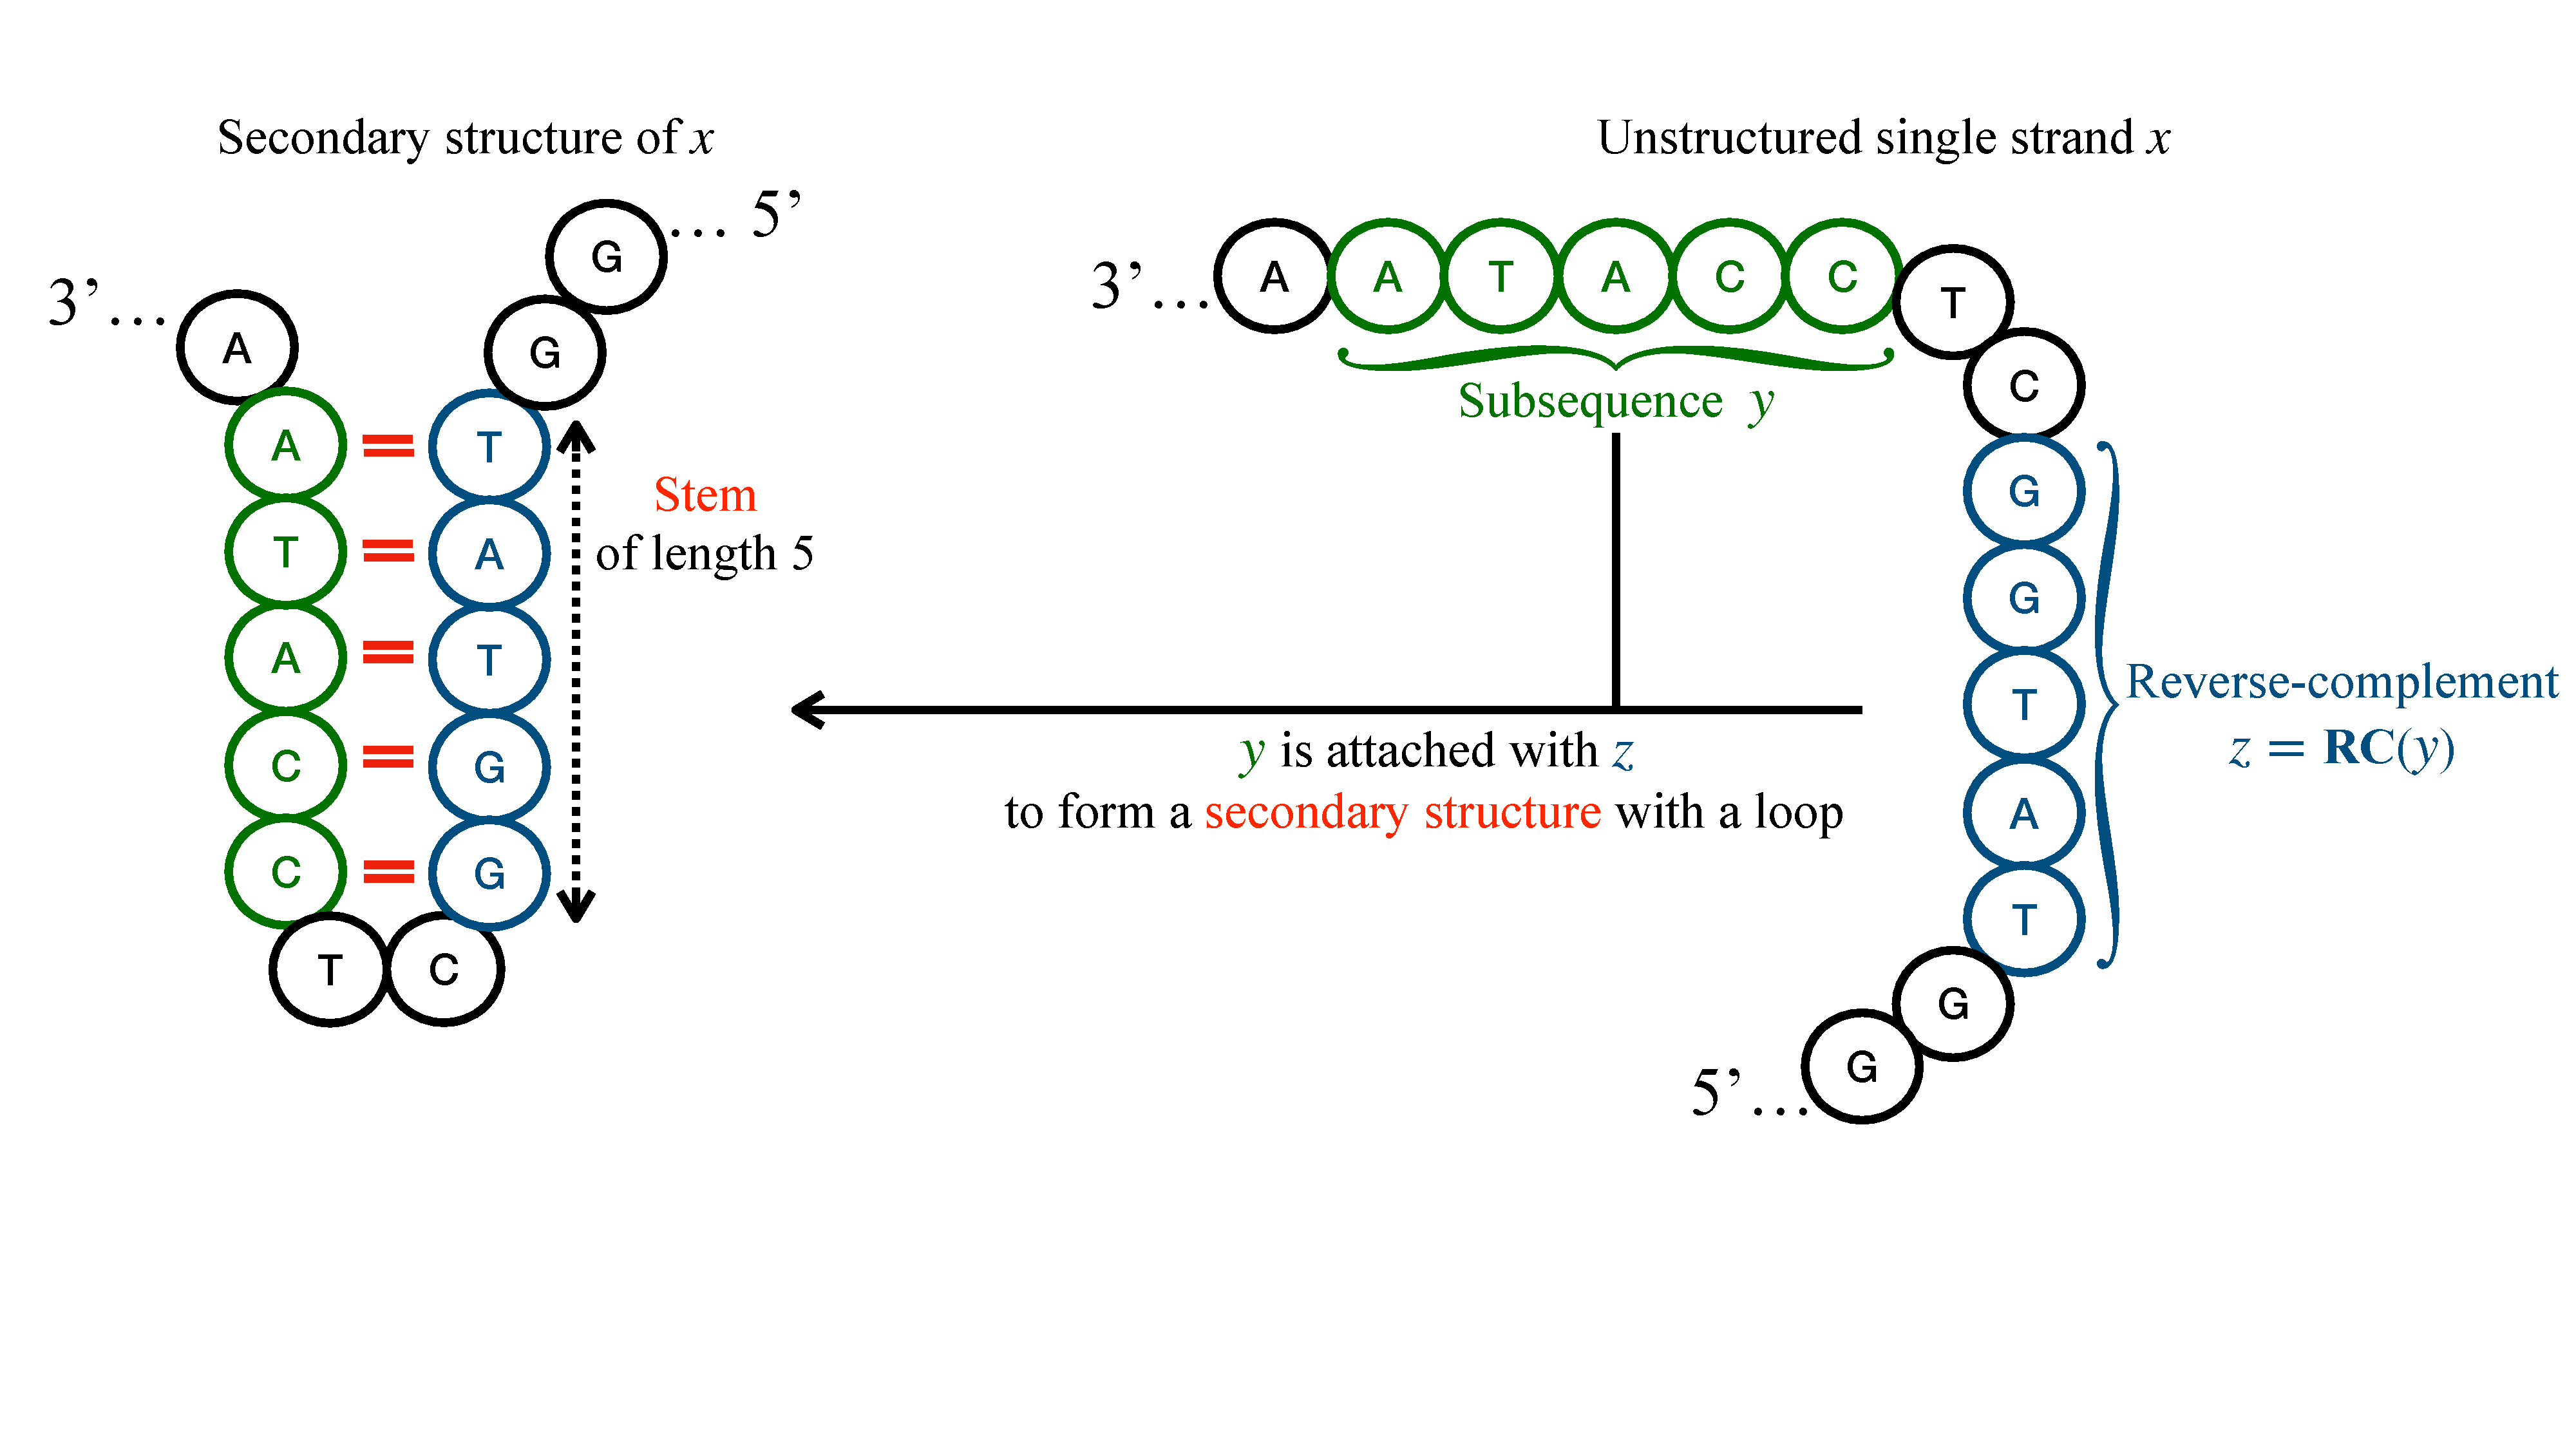
\includegraphics[width=9cm]{drawDNA3.pdf}
\end{center}
%\begin{center}
%\includegraphics[width=14cm]{drawDNA1.pdf}
%\end{center}
\caption{DNA secondary structure model. Here, the Watson-Crick complement is: $\overline{{\bf A}}={\bf T}, \overline{\bf T}={\bf A}, \overline{\bf C}={\bf G}$, and $\overline{\bf G}={\bf C}$.}
\label{fig1}
\end{figure*}


%\begin{figure}[t]
%\centering 
%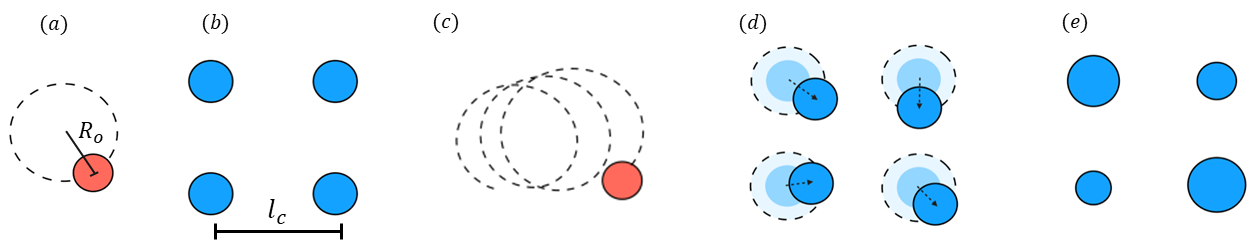
\includegraphics[width=8cm]{fig_1.eps}
%\caption{LALALA}
%\centering 
%\end{figure}


It has been shown experimentally that the number of base pairs in stem regions (or {\em stem length}) is one important factor influencing the secondary structure of a DNA sequence. Given codeword length $n$ and an integer $m\ge 2$, we study the problem of constructing DNA codes of length $n$ that avoid secondary structure of any stem length more than or equal to $m$. To the best of our knowledge, this work is the first attempt aimed at providing a rigorous solution for DNA codes avoiding secondary structure for general stem lengths.
%cases of stem length. 
%Construction of DNA codes, satisfy multiple constraints, are also discussed. 

%Motivated by this property, the main contribution of this work is to provide an explicit construction of DNA codes that completely avoid secondary structure of arbitrary stem length. 


%Formally, given codeword length $n$ and arbitrary integer $m\ge 2$, we provide efficient methods to construct DNA codes of length $n$ that avoid secondary structure of any stem length more than or equal to $m$. While there exists only explicit constructions of codes for $m=3$ in the literature, this work is the first attempt aimed at providing a rigorous solution for DNA codes avoiding secondary structure for general cases of stem length. Construction of DNA codes, besides avoiding secondary structure, also satisfy the {\bf G}{\bf C}-content constraint, are also presented. 


%It has been shown experimentally that the most important factors influencing the secondary structure of a DNA sequence are the number of base pairs in stem regions, the number of base pairs in a hairpin loop region as well as the number of unpaired bases. 

%The secondary structure refers to the tendency of a single-stranded DNA sequence to fold back upon itself, thus becoming inactive in the computation process.

%In addition, various combinations of these properties have been considered in \cite{K:2021,KDG:2021,O2:2005,TT:2021}.

 

%It was observed in [6] that the stability of duplexes depends on the combinatorial structure of the sequences, more precisely, on the combination of adjacent pairs of bases present in the oligonucleotide strands.

\section{Preliminary}\label{sec:prelim}
%\subsection{Secondary Structure Avoidance Codes}
In this work, we use $\D$ to denote the DNA alphabet, where $\D=\{{\bf A}, {\bf T}, {\bf C}, {\bf G}\}$. Here, we have the Watson-Crick complement where $\overline{{\bf A}}={\bf T}, \overline{\bf T}={\bf A}, \overline{\bf C}={\bf G}$, and $\overline{\bf G}={\bf C}$. 

Given two sequences $\bx$ and $\by$, we let $\bx\by$ denote the {\em concatenation} of the two sequences. 

Throughout this work, given a sequence $\bx$ of length $n$, we say $\by$ is a subsequence of length $k$ of $\bx$, where $k\le n$, if $\by=x_ix_{i+1}\ldots x_{i+k-1}$ for some $1\le i\le n-k+1$. In other words, we only consider the subsequences including consecutive symbols in $\bx$. Two subsequences $\by$ and $\bz$ of $\bx$ are said to be {\em non-overlapping} if we have $\by=x_ix_{i+1}\ldots x_{i+k-1}$, $\bz=x_jx_{j+1}\ldots x_{j+\ell-1}$, where $i>j+\ell-1$ or $j>i+k-1$.

%In this work, we use $\D$ to denote the DNA alphabet, where $\D=\{{\bf A}, {\bf T}, {\bf C}, {\bf G}\}$. 
%In the special case where $\bx,\by$ are of same length $n$, we use $\bx || \by$ to denote their {\em interleaved sequence}, i.e. $\bx || \by=x_1y_1x_2y_2\ldots x_ny_n$.
%In DNA storage, digital data is converted to quaternary alphabet according to the following rule, $ {\bf A}\leftrightarrow 00, {\bf T} \leftrightarrow 01, {\bf C} \leftrightarrow 10, {\bf G} \leftrightarrow 11$. Therefore, given a DNA sequence $\bx$ over the DNA alphabet $\D=\{{\bf A}, {\bf T}, {\bf C}, {\bf G}\}$ of length $n$, we have a corresponding a binary sequence $\Psi(\bx)\in\{0,1\}^{2n}$.

\begin{definition}
For a DNA sequence $\bx \in \D^n$, $\bx=x_1x_2\ldots x_n$, the reverse-complement of $\bx$, is defined as ${\rm RC}({\bx})={\overline{x_n}} \text{ } \overline{x_{n-1}}\ldots  \overline{x_3}  \text{ } \overline{x_2}  \text{ } \overline{x_1}$. %Here, we have the Watson-Crick complement where $\overline{{\bf A}}={\bf T}, \overline{\bf T}={\bf A}, \overline{\bf C}={\bf G}$, and $\overline{\bf G}={\bf C}$. %Over the binary alphabet, we have $\overline{0}=1$ and $\overline{1}=0$.
\end{definition}

%Throughout this work, given a sequence $\bx$ of length $n$ over alphabet $\Sigma$, we say $\by$ is a subsequence of length $k$ of $\bx$, where $k\le n$, if $\by=x_ix_{i+1}\ldots x_{i+k-1}$ for some $1\le i\le n-k+1$. In other words, we only consider the subsequences including consecutive symbols in $\bx$. Two subsequences $\by$ and $\bz$ of $\bx$ are said to be {\em non-overlapping} if we have $\by=x_ix_{i+1}\ldots x_{i+k-1}$, $\bz=x_jx_{j+1}\ldots x_{j+\ell-1}$, where $i>j+\ell-1$ or $j>i+k-1$.
\begin{definition}
Given $0<m\le n$, a DNA sequence $\bx\in \D^n$ is said to be $m$-secondary structure avoidance (or $m$-SSA) sequence if for all $k\ge m$, there does not exist any pair of non-overlapping subsequences $\by, \bz$ of length $k$ of $\bx$ such that $\by={\rm RC}({\bz})$. A code $\C$ is said to be an $(n,\D;m)$ SSA code if for every codeword $\bx\in \C \cap \D^n$, we have $\bx$ is $m$-SSA. 
\end{definition}

The following result is immediate. 
\begin{lemma}\label{lemma1}
Given $m,n>0$, if a sequence $\bx\in \D^n$ is  $m$-SSA then $\bx$ is $m'$-SSA for all $m'>m$. 
\end{lemma}

%However, the converse is not true. 
%\begin{example}
%Suppose that $\bx= {\color{ForestGreen}{{\bf A}{\bf C}{\bf G}}}{\bf G} {\color{blue}{{\bf C}{\bf G}{\bf T}}}{\bf G}$. We observe that $\bx$ is 4-SSA, but $\bx$ is not 3-SSA since there exists $\by={\color{ForestGreen}{{\bf A}{\bf C}{\bf G}}}$ and $\bz= {\color{blue}{{\bf C}{\bf G}{\bf T}}}$ in $\bx$ where $\by={\rm RC}({\bz})$.
%\end{example}

For a code $\C \subseteq \D^n$, the {\em code rate} is measured by the value $\log |\C|/n$. Intuitively, it measures the number of information bits stored in each DNA symbol.  Suppose that we have an infinite family of codes $\{\C_n\}_{n=1}^\infty$, where $\C_n$ is a code of length $n$, then the asymptotic rate of the family is ${\bf r} \triangleq \lim_{n\to \infty} \frac{\log |\C_n|}{n}$. Here, we adopt the notation $\log$ to mean logarithm base two. %


%In this work, we also study the channel capacity and provide some bounds. 

\begin{definition} 
Given $m>0$, for $n>0$, let ${\rm A}(n,\D;m)$ be the total number of DNA sequences of length $n$ that are $m$-SSA. The channel capacity, denoted by ${\rm c}_m$, is defined by: 
\begin{small}
\begin{equation*} 
{\rm c}_m=\lim_{n \to \infty} \frac{\log {\rm A}(n,\D;m)}{n}.
\end{equation*}  
\end{small}
\end{definition}

The following result is immediate. 

\begin{lemma}\label{trivial-bound} 
Given $m>0$, let $S_m$ be the set of all DNA sequences of length $m$ such that, there is no pair of sequences $\by, \bz \in S_m$, not necessary distinct, such that $\by={\rm RC}(\bz)$. We then have ${\rm c}_m \le 1/m \log |S_m|$. 
\end{lemma}

Observe that the size of $S_m$ can be computed easily for constant $m$, a trivial upper bound is that $|S_m| \le 4^m/2$, and consequently, we obtain ${\rm c}_2 \le 1.5$ and ${\rm c}_3 \le 1.67$. 

To construct an $(n,\D;m)$ SSA code for arbitrary $m>0$ by concatenation method, one can find the largest set $S_N$ for some suitable value of $N$, such that, for $n=Nk$, each codeword is a concatenation of $k$ sequences of length $N$ from $S_N$ and each concatenation does not create a reverse-complement subsequence from previous concatenations. The construction yields a family of DNA codes of rate $1/N \log |S_N|$ bits/nt. For example, for $m=3$, Krishna Gopal Benerjee and Adrish Banerjee \cite{K:2021} constructed an $(n,\D;3)$ SSA code via such a set $S=\{{\bf A}{\bf A}, {\bf C}{\bf C}, {\bf A}{\bf C}, {\bf C}{\bf A},{\bf T}{\bf C}\}$. 
%Based on the Nussinov-Jacobson (NJ) algorithm in \cite{RN:1980}, Olgica Milenkovic and Navin Kashyap in \cite{O2:2005, O:2005} found some design criteria that reduce the possibility of secondary structure formation in a codeword. Recently, Krishna Gopal Benerjee and Adrish Banerjee \cite{K:2021} provided an explicit construction for $3$-SSA DNA codes, based on the concatenation method. 

%where each codeword is the concatenation of words of length two from the set $S=\{{\bf A}{\bf A}, {\bf C}{\bf C}, {\bf A}{\bf C}, {\bf C}{\bf A},{\bf T}{\bf C}\}$. 

\begin{theorem}[Benerjee and Banerjee \cite{K:2021}]
Set $S=\{{\bf A}{\bf A}, {\bf C}{\bf C}, {\bf A}{\bf C}, {\bf C}{\bf A},{\bf T}{\bf C}\}$. Let $\C$ be the DNA code of length $2n$ where each codeword is a concatenation of words of length two from $S$. We then have $\C$ is an $(n,\D;3)$ SSA code, i.e. every codeword of $\C$ is $3$-SSA. The size of the code is $|\C|=5^n$, and the code rate is $1/2 \log 5 = 1.1609$ bits/nt.  
\end{theorem}

\subsection{Paper Organisation and Our Main Contribution}

Since the number of base pairs in stem regions (or stem length) is one important factor influencing the secondary structure of a DNA sequence, this work aims at providing a rigorous solution for $(n,\D;m)$ SSA codes given arbitrary $m$. 
%\subsection{Our Contribution} 
%The main contributions of this paper is to provide an explicit construction of DNA codes that completely avoid secondary structure of arbitrary stem length. Particularly, when $m=3$, our constructions yield a family of DNA codes of rate 1.303 bits/nt, which is higher than the code rate in \cite{K:2021}.
%\subsection{Paper Organisation and Our Main Contribution}
The paper is organised as follows. 
\begin{itemize}
\item Section III presents two efficient constructions of  $(n,\D;m)$ SSA codes for arbitrary $m>0$. The first construction is based on {\em block concatenation}, which concatenates blocks of fixed length $m$ from a predetermined set. On the other hand, crucial to the second construction is the concept of {\em symbol-composition constrained codes}. Particularly, when $m = 3$, the second construction yields a family of DNA codes of rate $1.3031$ bits/nt, which is higher than the code rate in \cite{K:2021}. 
%{\color{red}{We also study the channel capacity and present capacity-achieving codes when $m=2$.}} 
%done recursively to the length of codeword $n$
\item Section IV presents a linear-time encoding method for $(n,\D;m)$ SSA code with only one redundant symbol whenever $m\ge 3 \log n+4$. The coding method is based on {\em sequence replacement technique}. %We also show that our method can be further extended to design DNA codes combatting multiple constraints. For certain code parameters, our method incurs at most one redundant symbol.
%such as ${\bf G}{\bf C}$-content constraint, runlength limited constraint, Hamming distance constraint. For certain code parameters, our method incurs at most one redundant symbol.

%\item Section V provides efficient design of DNA codes combatting multiple constraints, where each DNA codeword is $\epsilon$-balanced, and $m$-SSA for arbitrary value of $\epsilon$, and $m$. Particularly, for certain values of $m,\epsilon$, and for sufficiently large $n$, our method incurs at most one redundant symbol. 
%\item Section VI Provides efficient design of DNA constrained codes with error-correction capability. Our codebook is capable of correcting a combination of deletions, insertions and substitutions, which are the most common errors in DNA-based data storage channel. 
\end{itemize}




\section{Constructions of $(n,\D;m)$ SSA Codes for arbitrary $m>0$} 
%\hm{The second construction is not really concatenation. Maybe ``Constructions for fixed $m$''?}
The first method is based on block concatenation, which concatenates blocks of length $m$ from a predetermined set.
%In this section, we presents the explicit construction for $m$-SSA $\C(n,\D;m)$ DNA codes for arbitrary $m>0$ based on concatenation coding method. 
\begin{comment}
{\color{red}{We first present the capacity-achieving codes when $m=2$.

\subsection{Capacity-Achieving Codes when $m=2$}
\begin{lemma}\label{m2}
Set $\D'=\{{\bf A}, {\bf G}\}$. For $n>0$, let $\C$ be the DNA code of length $n$ over the alphabet $\D'$. We then have $\C$ is $2$-SSA DNA code. The size of the code is $|\C|=2^n$, and the code rate is $1$ bits/nt.
\end{lemma}

\begin{lemma}[capacity bound]
We have $1\le c_2 \le 1.292$.
\end{lemma}

\begin{proof}
The lower bound follows from Lemma~\ref{m2} while the upper bound follows from Lemma~\ref{trivial-bound}, where $S_2=\{{\bf A}{\bf A}, {\bf A}{\bf C}, {\bf C}{\bf A}, {\bf C}{\bf C}, {\bf A}{\bf G}, {\bf T}{\bf C} \}$. 
\end{proof}

\begin{conjecture}
We have $c_2=1$. 
\end{conjecture}

\begin{proof}
Use finite states machine. 
\end{proof}


}}

\end{comment}
\subsection{Constructions via Block Concatenation}
%\hm{Shall we call this method ``Block Concatenation''? Actually, Immink refers to such constructions as block encoders in his text.}
\begin{construction}\label{fixed-concatenate}
Given $m>0$, $n=mk$ for some integer $k>0$, set $t=\ceil{m/3}$. Let $S_m^*$ be the set of all DNA sequences of length $m$ such that for any pair of sequences $\bx_1,\bx_2 \in S_m^*$, not necessary distinct, there is no pair of subsequences $\by$ of $\bx_1$ and $\bz$ of $\bx_2$ of length $t$ such that $\by={\rm RC}(\bz)$. Let $\C$ be the DNA code of length $n$, where each codeword is a concatenation of $k$ sequences of length $m$ in $S_m^*$.
\end{construction} 

\begin{theorem}\label{con1}
The constructed code $\C$ from Construction~\ref{fixed-concatenate} is an $(n,\D;m)$ SSA code. 
\end{theorem} 

\begin{proof}
We prove the correctness of Theorem~\ref{con1} by contradiction. Suppose that, there exists a codeword $\bc\in \C, \bc=\bx_1\bx_2\ldots \bx_k$, where $\bx_i \in S_m^*$, and $\bc$ is not $m$-SSA. In other words, there exists two non-overlapping subsequences $\by$,$\bz$ of $\bc$ of length $m'\ge m$ such that $\by={\rm RC}(\bz)$. 

Suppose that $\by=Y_1 Y_2$ where $Y_1$ is a subsequence of $\bx_i$, and $Y_2$ is a subsequence of $\bx_{i+1}\bx_{i+2}\ldots \bx_{i+h}$ for some $h\ge 1$. We have $\bz={\rm RC}(Y_2) {\rm RC}(Y_1)$. The trivial case is if $h>1$, or $Y_2$ is of length more than $m$, then $\bx_{i+1}$ is a subsequence of $Y_2$ and $ {\rm RC}(\bx_{i+1})$ is a subsequence of $\bz$. Clearly, if $ {\rm RC}(\bx_{i+1}) \equiv \bx_j$, we have a contradiction. On the other hand, if $ {\rm RC}(\bx_{i+1})=W_1 W_2$ where $W_1$ is a subsequence of $\bx_j$ and $W_2$ is a subsequence of $\bx_{j+1}$ for some $j$, then at least one subsequence $W_1$ or $W_2$ is of size more than $t$, we also have a contradiction. We conclude that $h=1$, or $Y_2$ is simply a subsequence of $\bx_{i+1}$.

Now, since $\by=Y_1Y_2$ is of length $m'\ge m$, at least $Y_1\ge t$ or $Y_2\ge t$. W.l.o.g, assume that  $Y_1\ge t$.

%\item If $h>1$, or $Y_2$ is of length more than $m$, then $\bx_{i+1}$ is a subsequence of $Y_2$ and $ {\rm RC}(\bx_{i+1})$ is a subsequence of $\bz$. 
%Since $\by$ is of length $m$, one of the two subsequences $Y_1$, $Y_2$ is of length at least $t=\ceil{m/3}$. W. l. o. g, suppose that the length of $Y_1$ is more than or equal to $t$.  
We observe that ${\rm RC}(Y_1)$ cannot be a subsequence of any $\bx_j$ by Construction 1. In other words, ${\rm RC}(Y_1)=W_1 W_2$ where $W_1$ is a subsequence of $\bx_j$ and $W_2$ is a subsequence of $\bx_{j+1}$ for some $j$. Similarly, we observe that the length of $W_1, W_2$ must be strictly smaller than $t$, otherwise, for example, if the length of $W_1$ is more than or equal to $t$, then two sequences $\bx_i$ and $\bx_j$ in $S_m^*$ contain ${\rm RC}(W_1)$ and $W_1$ as subsequences, we have a contradiction. Since both the length of $W_1, W_2$ must be strictly smaller than $t$, causing the length of $Y_1$ is smaller than $2t$, we conclude that the length of $Y_2$ is at least $t$. 

Now, let $\bU={\rm RC}(Y_2) \cap \bx_{j+1}$, the subsequence that belongs to both $\bx_{j+1}$ and ${\rm RC}(Y_2)$, which is of size at least $t$. We then have $\bU$ is a subsequence of $\bx_{j+1}$ while ${\rm RC}(\bU)$ is a subsequence of ${\rm RC}({\rm RC}(Y_2))=Y_2$, a subsequence of $\bx_{i+1}$. We then have a contradiction. 

In conclusion, we have $\C$ is an $(n,\D;m)$ SSA code. We highlight our proof sketch of Theorem~\ref{con1} in Figure~\ref{fig2}.
\end{proof}
\begin{figure}[h]
\caption*{Claim 1: When $|Y_1|\ge t$, we observe that ${\rm RC}(Y_1)$ cannot be a subsequence of any $\bx_{j+1}$.}
\begin{center}
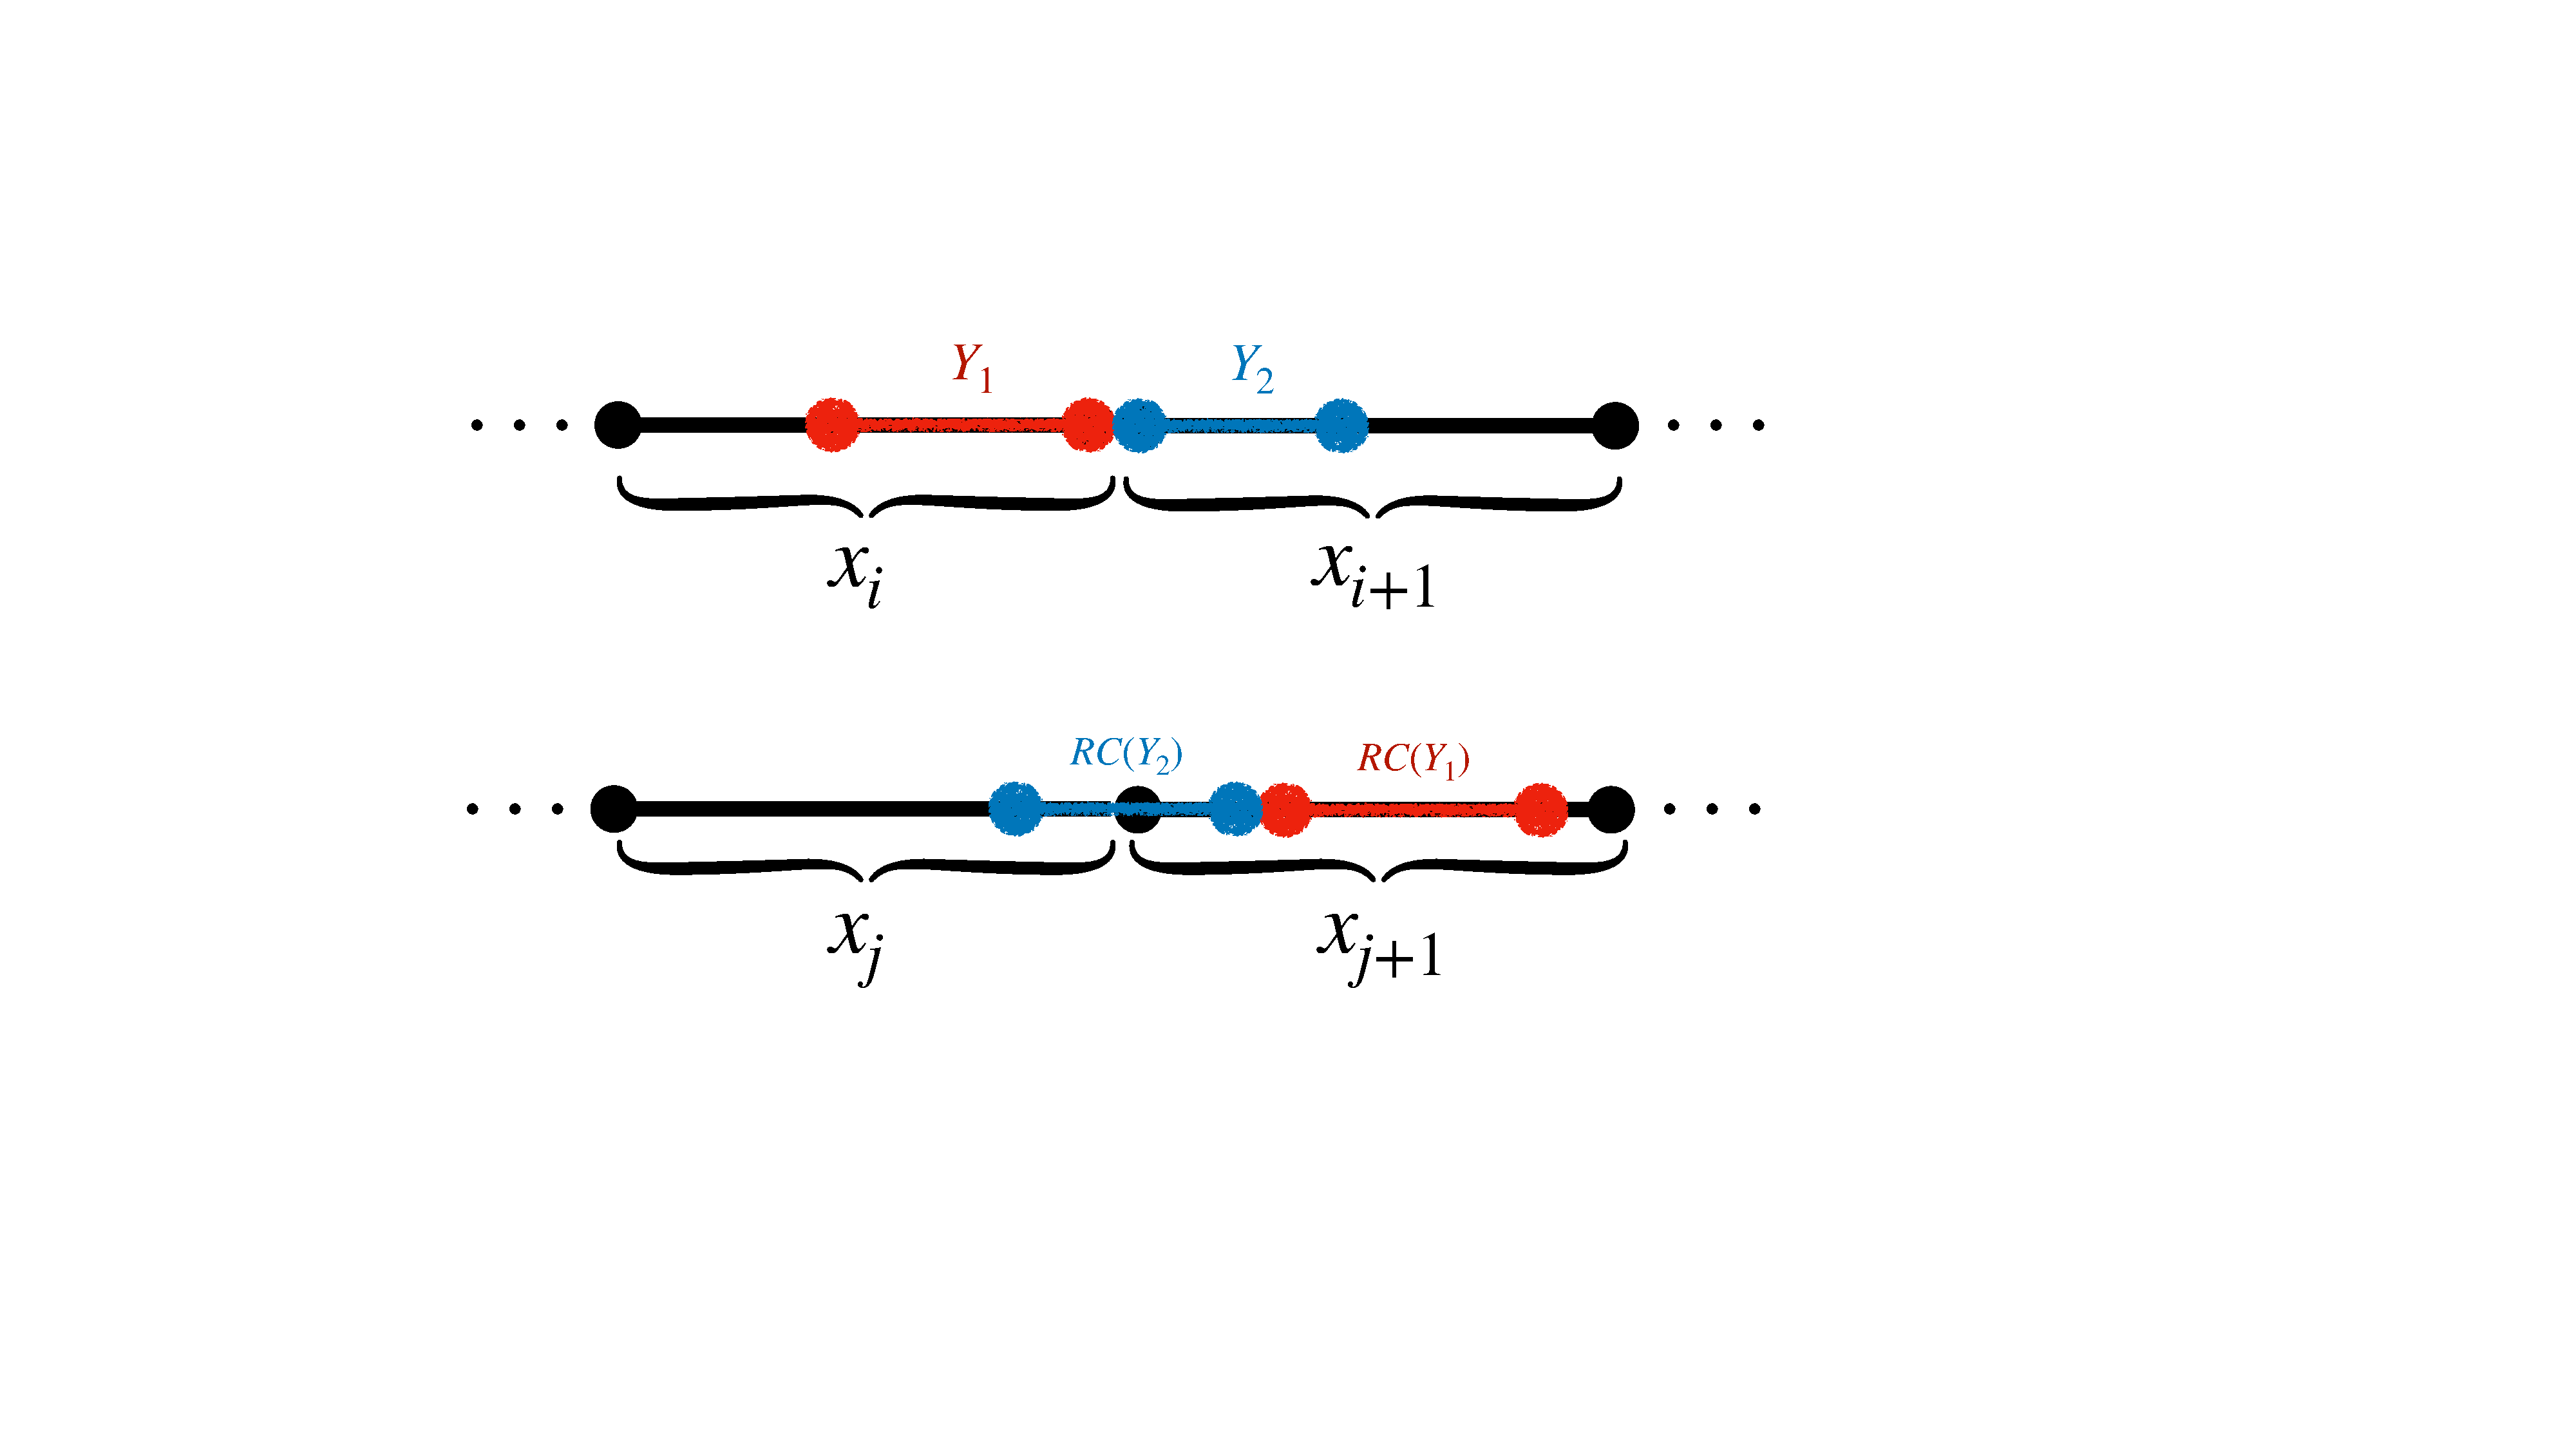
\includegraphics[width=5.5cm]{proof2.pdf}
\end{center}
\caption*{Claim 2: When $Y_1=W_1W_2$ and ${\rm RC}(Y_1)={\rm RC}(W_2){\rm RC}(W_1)$, we must have $|W_1|\le t, |W_2|\le t$.}
\begin{center}
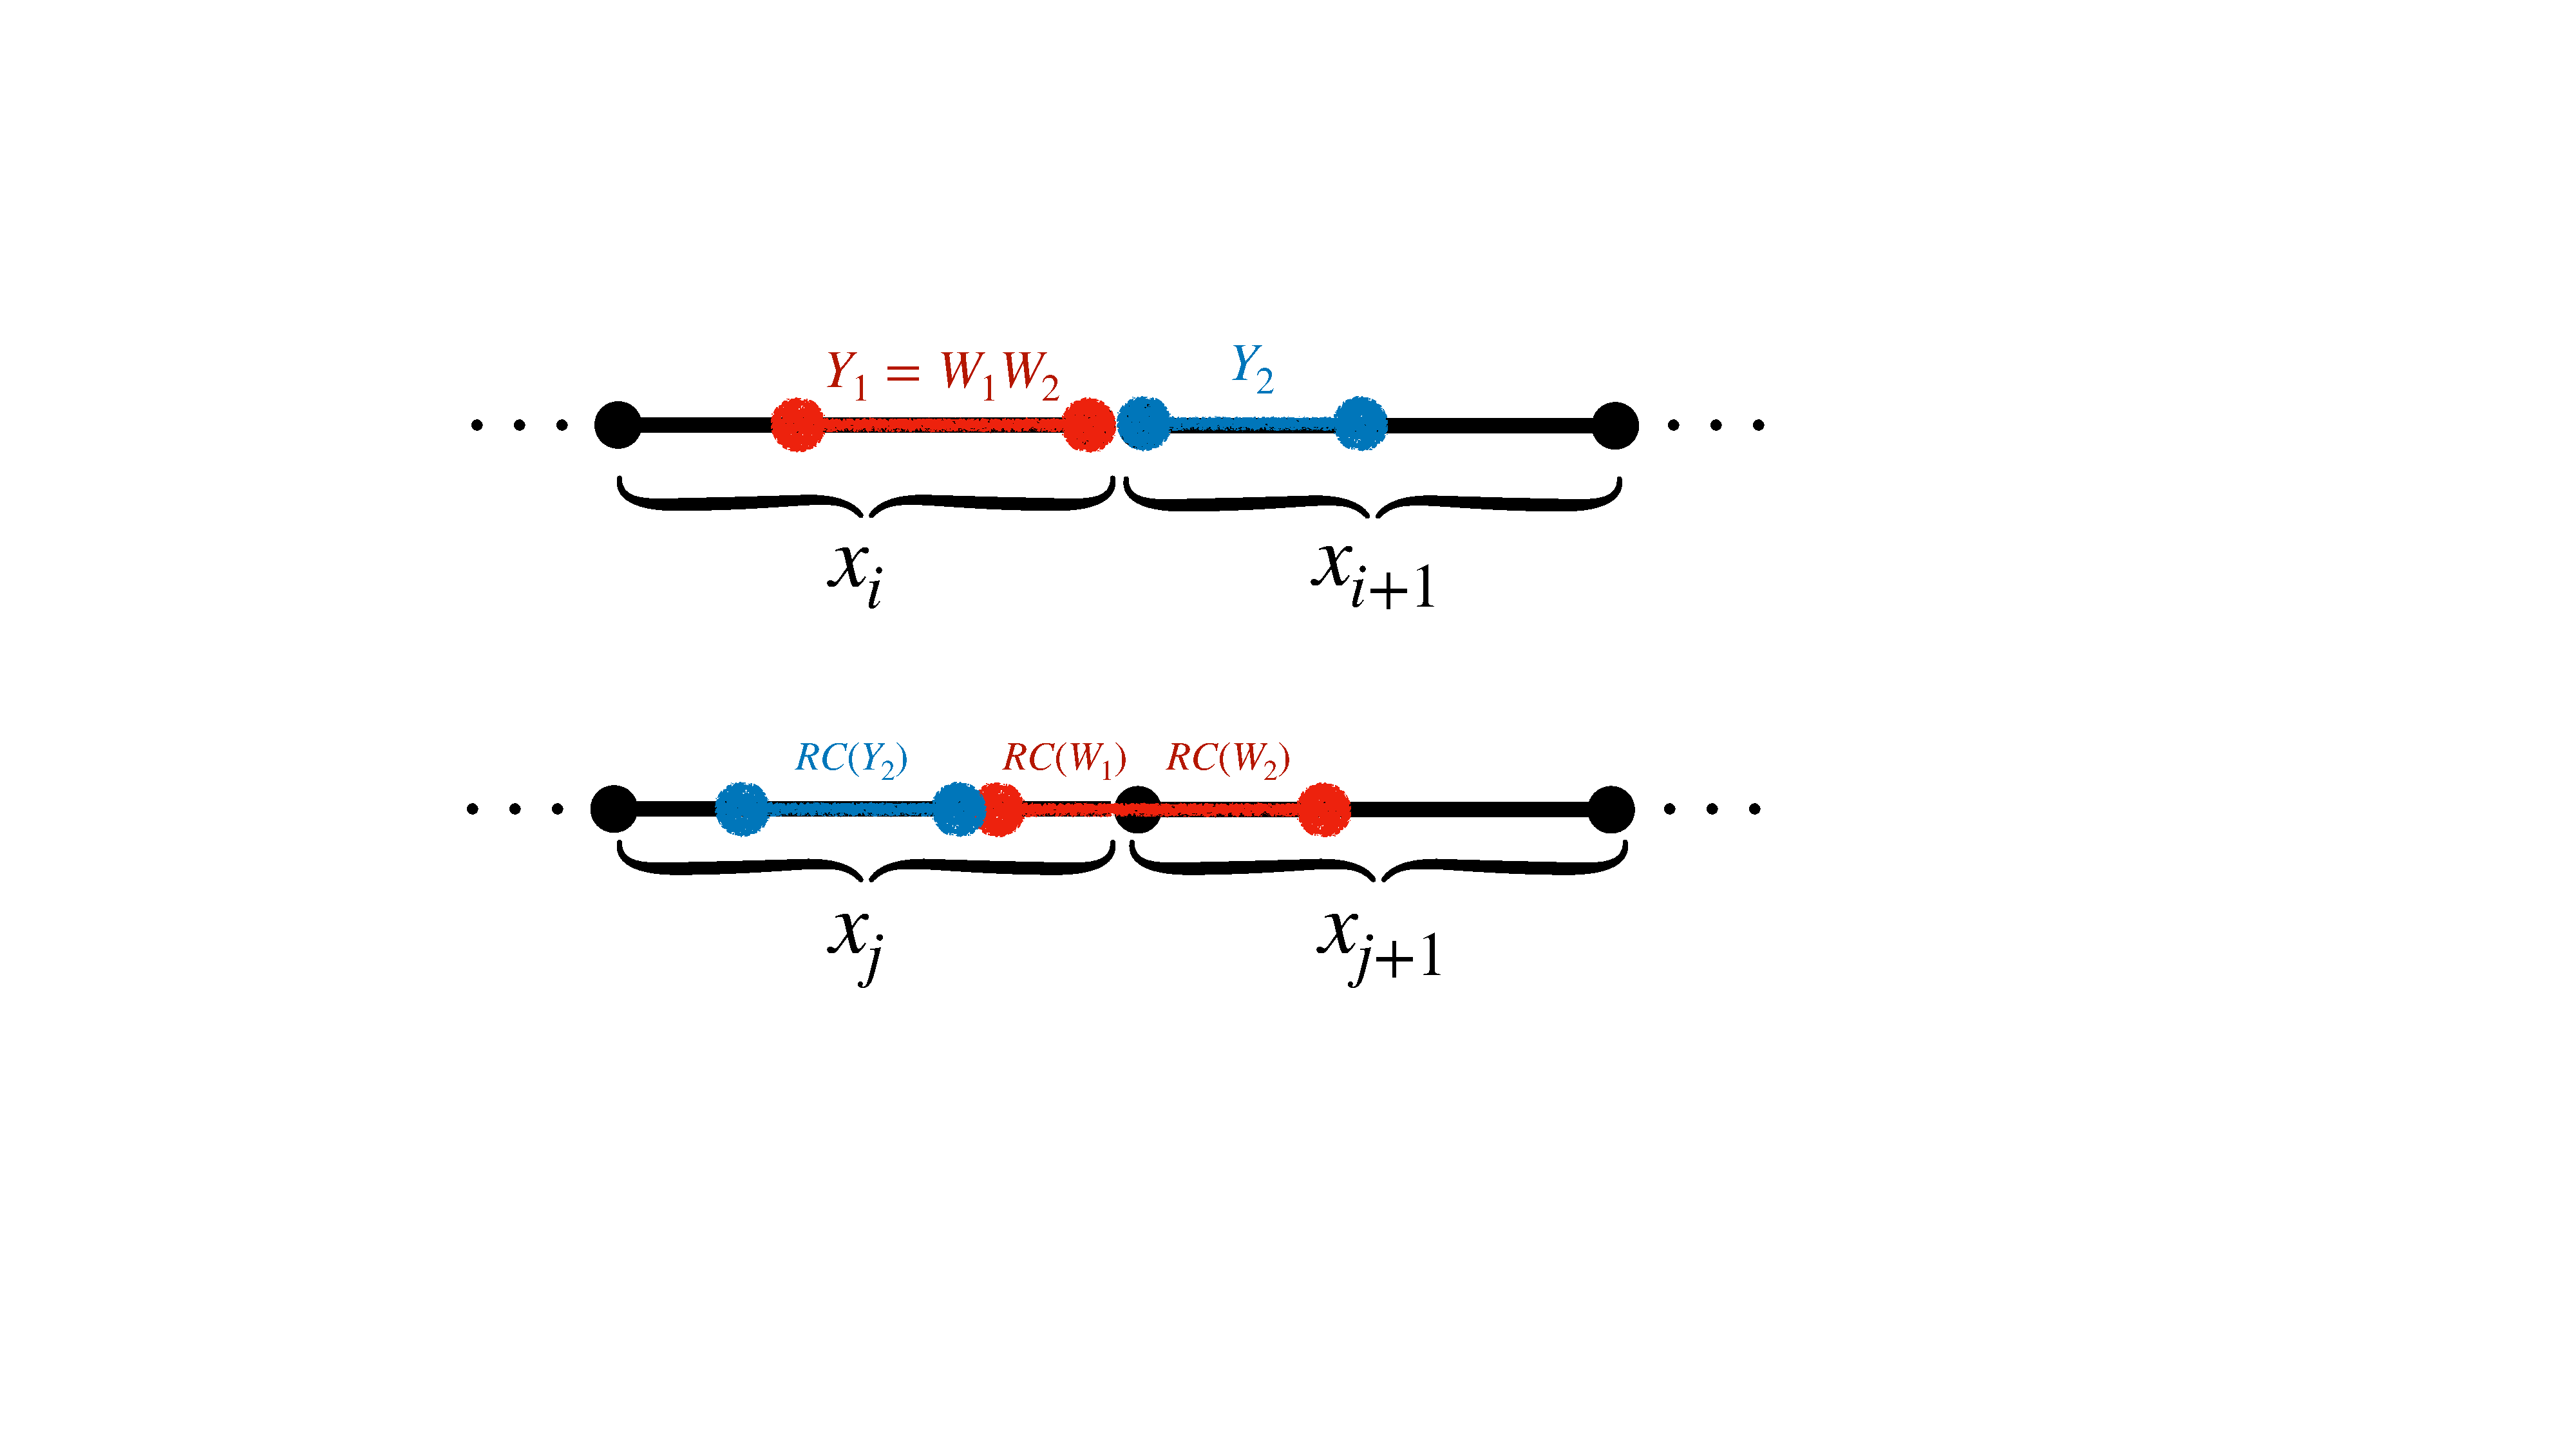
\includegraphics[width=6cm]{proof1.pdf}
\end{center}
\caption*{Consequently, $|Y_2| \ge t$, and we have $(\bx_{i+1},\bx_j)$ form a pair in $S_m^*$ that violate the condition.}
\caption{Proof Sketch of Theorem~\ref{con1}.}
\label{fig2}
\end{figure}
\begin{remark} Observe that, the set $S_m^*$ can be constructed via exhaustive search with complexity $O(2^m)$. In Section IV, we show that when $m$ is sufficiently large, $m\ge 3\log n+4=\Theta(\log n)$, there exists an efficient encoding/decoding algorithm for $(n,\D;m)$ SSA codes with at most one redundant symbol. Hence, for the case $m=o(\log n)$, we can use Construction~\ref{fixed-concatenate} to construct $(n,\D;m)$ SSA codes with complexity $2^m=\Theta(n)$. %In addition, it is easy to see that Construction~\ref{fixed-concatenate} works for any set $S_M^*$ where $M\ge m$. 
\end{remark} 
\begin{comment}
It is easy to see that Construction~\ref{fixed-concatenate} works for any set $S_M^*$ where $M\ge m$. 
\begin{corollary}\label{coro1} 
Given $m>0$, set $t=\ceil{m/3}$. For $M\ge m$, let $S_M^*$ be the set of all DNA sequences of length $M$ such that for any pair of distinct sequences $\bx_1,\bx_2 \in S_M^*$, there is no pair of subsequences $\by$ of $\bx_1$ and $\bz$ of $\bx_2$ of length $t$ such that $\by={\rm RC}(\bz)$. Let $\C'$ be the DNA code of length $n$, where each codeword is a concatenation of $k$ sequences of length $M$ in $S_m^*$. We then have $\C'$ is $m$-SSA DNA code.
\end{corollary}
\end{comment}
%{\color{purple}{
%\begin{remark} (To be edited) Observe that the set $S_m^*$ can be constructed easily for constant $m$ via exhaustive search. In Section IV, we show that when $m \ge 1.5\log n+2$, there exists an efficient encoding/decoding algorithm for $m$-SSA DNA code with at most one redundant symbol. Hence, for the case $m <  1.5\log n+2$ or $m=o(\log n)$, we can use Construction 1 to construct $m$-SSA DNA code with complexity at most $2^m=2^{o(\log n)}=\Theta(n)$. 
%\end{remark} 
%}}


\subsection{Constructions via Symbol-Composition Constrained Codes}
%\hm{Shall we refer to this as ``Sliding-Window-Constrained Codes'' }
In this subsection, we present an efficient construction for $(n,\D;m)$ SSA codes 
%via recursive concatenation. 
by simply restricting the symbol-composition for every subsequence of length $m$. Particularly, when $m = 3$, our method yields a family of DNA codes of rate $1.3031$ bits/nt, which is higher than the code rate in \cite{K:2021}. 
\vspace{0.05in}

%\noindent{\em A natural idea.} 
\noindent{\em High Level Description}.
We select a nucleotide $x \in \D=\{{\bf A}, {\bf T}, {\bf C}, {\bf G}\}$, and let $y=\overline{x}\in \D$. For some $0<k\le m$, we present an efficient method to construct an $(n,\D;m)$ SSA code $\C$ as follows. For every codeword $\bc\in\C$, every subsequence $\bz$ of length $m$ of $\bc$ contains at least $k$ symbols $x$ while $\bz$ contains at most $(k-1)$ symbols $y$. We refer such a constraint to as the {\em symbol-composition constraint}. 
It is easy to verify that such a constructed code $\C$ is an $(n,\D;m)$ SSA code. Clearly, suppose on the other hand, there exists a pair of subsequences $\bz_1, \bz_2$ of length $\ell\ge m$ in $\bc\in \C$, such that $\bz_2={\rm RC}(\bz_1)$. It implies that there exists two subsequences of length $m$, which are $\bz_1'$ of $\bz_1$ and $\bz_2'$ of $\bz_2$, and $\bz_2'={\rm RC}(\bz_1')$. Since $\bz_1'$ contains at least $k$ symbols $x$, we have $\bz_2'={\rm RC}(\bz_1')$ must contain at least $k$ symbols $y=\overline{x}$. We then have a contradiction.
\vspace{0.05in}

The following construction is for $m=3$ and $k=1$.

%\begin{construction}[Recursive Construction for $m=3$, $k=1$]\label{con2}
\begin{construction}[Symbol-Composition Constrained Codes for $m=3$, $k=1$]\label{con2}
Given $n>0$, we select $x={\bf A}$ and $y=\overline{x}={\bf T}$. Set $\D^*=\{{\bf A}, {\bf C}, {\bf G}\}$. Let $\C_n$ be the set of all DNA sequences of length $n$ from alphabet $\D^*$ such that for any $\bc\in\C_n$, every subsequence of length three of $\bc$ must contain an ${\bf A}$. 
\end{construction}

\begin{theorem} We have $|\C_1|=3, |\C_2|=9,|\C_3|=19$, and
\begin{equation*}
|\C_n|= |\C_{n-1}| + 2| \C_{n-2}| + 4 |\C_{n-3}|.
%|\C_n|= \C_{n-1} {\bf A} \cup  \C_{n-2} {\bf A}{\bf C} \cup \C_{n-2} {\bf A}{\bf C} 
\end{equation*}  
In addition, $\C_n$ is an $(n,\D;3)$ SSA code for all $n>0$. The asymptotic rate of this code family is given by $\log (\lambda) \approx 1.3031$, where $\lambda\approx 2.4675$ is the largest real root of $x^3-x^2-2x-4=0$.
\end{theorem}

\begin{proof}
Consider the code $\C_n$. For a codeword $\bc \in \C_n$, for any subsequence $\bx$ of length $\ell \ge 3$ of $\bc$, we have $\bx$ includes ${\bf A}$. On the other hand, since $\overline{\bf A}={\bf T}$ is not used in $\bc$, there is no reverse-complement of $\bx$ in $\bc$. In conclusion, $\bc$ is 3-SSA, or $\C_n$ is an $(n,\D;3)$ SSA code. 

We now prove the cardinality of  $\C_n$. it is easy to verify that $|\C_1|=3, |\C_2|=9,|\C_3|=19.$ For $n\ge 4$, we construct $\C_n$ recursively as
follows: 
\begin{small}
\begin{align*}
S^1_n=& \{ \bx {\bf A}: \text{ for } \bx \in \C_{n-1}\} \\
S^2_n=& \{ \bx {\bf A} {\bf C},  \bx {\bf A} {\bf G}: \text{ for } \bx \in \C_{n-2}\} \\
S^3_n=& \{ \bx {\bf A} {\bf C} {\bf C}, \bx {\bf A} {\bf C} {\bf G}, \bx {\bf A} {\bf G} {\bf C}, \bx {\bf A} {\bf G} {\bf G}: \text{ for } \bx \in \C_{n-3}\}, \text{and} \\
\C_n =& S^1_n \cup S^2_n \cup S^3_n.
\end{align*}
\end{small}
In other words, $S^1_n$ is the set formed by concatenating all sequences in $\C_{n-1}$ with ${\bf A}$, $S^2_n$ is the set formed by concatenating all sequences in $\C_{n-2}$ with ${\bf A}{\bf C}$ or ${\bf A}{\bf G}$, and lastly, $S^2_n$ is the set formed by concatenating all sequences in $\C_{n-3}$ with ${\bf A} {\bf C} {\bf C}, {\bf A} {\bf C} {\bf G}, {\bf A} {\bf G} {\bf C},$ or ${\bf A} {\bf G} {\bf G}$. It is easy to verify that $S^i_n \cap S^j_n\equiv \emptyset$, and the union $S^1_n \cup S^2_n \cup S^3_n$ includes all possible sequences in $\C_n$. Therefore, we have $|\C_n|= |\C_{n-1}| + 2| \C_{n-2}| + 4 |\C_{n-3}|.$
\end{proof}

Construction~\ref{con2} can be generalized to construct $(n,\D;m)$ SSA codes with $k=1$ as follows. 

%\begin{theorem}[Recursive construction for $m$-SSA, $k=1$]\label{con3}
\begin{theorem}[Symbol-Composition Constrained Codes for General $m$, $k=1$]\label{con3}
Given $n,m>0$. Set $\D^*=\{{\bf A}, {\bf C}, {\bf G}\}$, and $\C_n(m)$ to be the set of all sequences $\bx$ of length $n$ from alphabet $\D^*$ such that every subsequence of length $m$ of $\bx$ include an ${\bf A}$. We then have $|\C_i(m)|=3^i$ for $0\le i\le m-1$, and 
\begin{equation*}
|\C_n(m)|=\sum_{j=0}^{m-1} 2^j |\C_{n-j-1}(m)| \text{ for } n\ge m.
\end{equation*}
We then have $\C_n(m)$ is an $(n,\D;m)$ SSA code for all $n>0$. The asymptotic rate of this code family is given by $\log (\lambda)$, where $\lambda$ is the largest real root of $x^m-\sum_{j=0}^{m-1} 2^j x^{m-j}=0$.  
\end{theorem} 

\begin{remark} In general, given $m>k>0$, set $x={\bf A}$ and $y=\overline{x}={\bf T}$. we use $\C_n(m,k)$ to denote the set of all sequences $\bc\in\D^n$ such that every subsequence $\bz$ of length $m$ of $\bc$ contains at least $k$ symbols ${\bf A}$ while $\bz$ contains at most $(k-1)$ symbols ${\bf T}$. As shown earlier, $\C_n(m,k)$ is an $(n,\D;m)$ SSA code for all $m,k$. A natural question is, for a given number $m>0$, what is the value of $k$, where $1\le k\le m$, such that the code $\C_n(m,k)$ has the largest cardinality? We defer the study of $\C_n(m,k)$, including the code's cardinality and the design of efficient encoding algorithms to map arbitrary DNA sequences into such a code, to future research work. 
\end{remark}








\section{Constructions of $(n,\D;m)$ SSA Codes for $m\ge 3\log n+4$ with One Redundant Symbol} 

In this section, we show that when the stem length is sufficiently large, $m \ge 3\log n+4=\Theta(\log n)$, there exists an efficient encoding/decoding algorithm for $(n,\D;m)$ SSA codes with at most one redundant symbol. For simplicity, we assume that $\log_4 n$ is an integer, and define the {\em DNA-representation} of an integer as follows.  

%The Sequence Replacement Technique (SRT) has been widely applied in the literature (for example, see \cite{TT:2020,srt:2010,srt:2019,TT:2022}). This is an efficient method for removing forbidden substrings from a source word. The advantage of this technique is that the complexity of encoder and decoder is very low, and they are also suitable for parallel implementation. In general, the encoder removes the forbidden strings and subsequently inserts its representation (which also includes the position of the substring) at predefined positions in the sequence.

\begin{definition}
For a positive integer $N$, the {\em DNA-representation} of $N$ is the replacement of symbols in the quaternary representation of $N$ over $\Sigma_4 = \{0,1,2,3\}$ by the following rule:  $0  \leftrightarrow {\bf A}, 1  \leftrightarrow {\bf T}, 2  \leftrightarrow {\bf C}, \text{ and } 3  \leftrightarrow {\bf G}.$
\end{definition} 

\begin{example}
If $N=100$, the quaternary representation of length 4 of $N$ is $1210$, hence, the DNA-representation of $N$ is ${\bf T}{\bf C}{\bf T}{\bf A}$. Similarly, when $N=55$, the quaternary representation of length 4 of $N$ is $0313$, thus the DNA-representation of $N$ is ${\bf A}{\bf G}{\bf T}{\bf G}$.
\end{example}
\begin{comment}
It is an efficient method for removing forbidden subsequences from a source word. In general, the encoder removes the forbidden subsequence and subsequently inserts its representation (which includes its location) at predefined positions. The crucial steps in a coding method based on sequence replacement technique are as follows: 
\begin{itemize}
\item (P1) To ensure that the replacement procedure is guaranteed to terminate. A common idea, used in \cite{TT:2020, TT:2022, srt:2019}, is to replace each forbidden subsequence of length $\ell>0$ (if there is) with a subsequence of length shorter than $\ell$. Consequently, after each replacement step, the length of codeword is reduced, the replacement procedure is guaranteed to terminate. 
\item (P2) To ensure that the output codeword is of fixed-length. Since the number of replacement steps vary in different source sequences, it is crucial to design an efficient method that enables fixed-length output codewords. In general, for codewords of length $n$, if the length of the encoded sequence, after the replacement procedure, is $N_0$ where $N_0 < n$, it is necessary to append a suffix of length $N_1=n - N_0$ to obtain an output codeword of length $n$. In this work, the appending suffix should be constructed carefully so that it does not create any pair of subsequences that form a secondary structure. To overcome this challenge, we also restrict the length of the repeated patterns of size 2 (also known as {\em pattern length limited (PLL) constraint}, as introduced in \cite{{wang:2021}}).

%.maximum length of runs of repeated symbols (also known as {\em runlength limited constraint}).  
\end{itemize} 
 \end{comment}
%to ensure that the replacement procedure is guaranteed to terminate. The general idea is to replace each forbidden window of length  (if there is) with a subsequence of length shorter than . Consequently, after each replacement step, the length of codeword is reduced, the replacement procedure is guaranteed to terminate. In our problem, in the worst case, the final replacement step occurs when the length of the current word is  + 1, since after another replacement (if needed), the length of the current word becomes at most  and we cannot proceed further. This final step is crucial to ensure that the final output codeword satisfies the weight constraint. 

We now present explicit construction of the encoder $\enc_{{\rm SSA}}$ and the corresponding decoder $\dec_{\rm SSA}$. Our method is based on the sequence replacement technique. This method has been widely used in the literature \cite{TT:2020, TT:2022, srt:2019}. In addition, we also restrict the length of the repeated patterns of size 2 (also known as {\em pattern length limited (PLL) constraint}, as introduced in \cite{{wang:2021}}).
\vspace{0.05in}

\noindent{\bf Construction of $\enc_{{\rm SSA}}$}. Given $n>m>0$, $n> 16$, and $m\ge 3\log n+4$. Set $m'=1.5\log n+2$. The source DNA sequence $\bx \in \D^{n-1}$. The encoding algorithm includes three phases: {\em prepending phase}, {\em scanning and replacing phase}, and {\em extending phase}.
\vspace{0.05in}

\noindent{\em Prepending phase}. The source sequence $\bx\in\D^{n-1}$ is prepended with ${\bf A}$, to obtain $\bc={\bf A}\bx$ of length $n$. If $\bc$ is an $m$-SSA sequence, then the encoder outputs $\bc$. Otherwise, it proceeds to the next phase. %Suppose that $\bc=c_1c_2\ldots c_n$.
\vspace{0.05in} 

\noindent{\em Scanning and replacing phase}. The encoder searches for the first pair of non-overlapping subsequences $\by, \bz$ of length $\ell_1$ of $\bc$, where $\ell_1\ge m'$, such that $\by={\rm RC}(\bz)$, or the first subsequence $\bu$ of $\bc$ of the form $\bu=(x_1x_2)^t$ whose length is $\ell_2=2t \ge m'=1.5\log n+2$, where $x_1,x_2\in  \D=\{{\bf A},{\bf T},{\bf C},{\bf G}\}$.

\begin{itemize}
\item If it finds a pair of non-overlapping subsequences $\by, \bz$, suppose that $\bc=\bX_1 \by \bX_2 \bz \bX_3$, where $\bX_1, \bX_2, \bX_3$ are subsequences of $\bc$, and $\by$ starts at index $i$, ends at index $j$ in $\bc$, where $j=i+\ell_1-1$, and $\bz$ starts at index $k$ in $\bc$. We have $i,j,k \le n-1$. 
\vspace{0.05in}

{\em Type-I Replacement}. The encoder sets a pointer ${\rm P_I}$, starting with symbol ${\bf T}$, and ${\rm P_I}={\bf T} \bp_1 \bp_2 \bp_3$, where $\bp_1, \bp_2, \bp_3$ are the DNA-representation of $i, j,$ and $k$, respectively. Since $\bp_1, \bp_2, \bp_3$ are of length $\log_4 n$, the pointer sequence ${\rm P}_{\rm I}$ is of length $1+3\log_4 n=1+1.5 \log n$. It then removes $\bz$ from $\bc$ and prepends ${\rm P_I}$ to $\bc$. The replacing step can be illustrated as follows. 
\begin{equation*}
 \bX_1 {\color{blue}{\by}} \bX_2 {\color{blue}{\bz}} \bX_3 \to \bX_1 {\color{blue}{\by}} \bX_2 \bX_3 \to {\color{red}{{\bf T} \bp_1 \bp_2 \bp_3}} \bX_1 {\color{blue}{\by}} \bX_2 \bX_3
\end{equation*}
Noted that the removed sequence $\bz$ is of length $\ell_1 \ge m' = 1.5 \log n+2$, while the insertion pointer ${\rm P}_I$ is of length $1.5 \log n+1$. Consequently, such a replacement reduces the length of the current sequence by at least one symbol. 

\item On the other hand, suppose that it finds a subsequence $\bu$ of $\bc$ of the form $\bu=(x_1x_2)^t$ whose length is $\ell_2=2t \ge m'$, where $x_1,x_2\in  \D=\{{\bf A},{\bf T},{\bf C},{\bf G}\}$. We further suppose that $\bc=\bU_1 (x_1x_2)^{t} \bU_2$, where $\bU_1, \bU_2$ are subsequences of $\bc$, and $\bu$ starts at index $i$, and ends at index $j$ in $\bc$, where $j=i+\ell_2-1$. We have $i,j \le n-1$.
\vspace{0.05in}

{\em Type-II Replacement}. Similarly, the encoder sets a pointer ${\rm P_{II}}$, starting with symbol ${\bf C}$, and ${\rm P_{II}}={\bf C} x_1 x_2 \bq_1 \bq_2$, where $\bq_1, \bq_2$ are the DNA-representation of $i$ and $j$, respectively. Since $\bq_1, \bq_2$ are of length $\log_4 n$, the pointer sequence ${\rm P_{II}}$ is of length $1+2+2\log_4 n=3+\log n$. It then removes $(x_1x_2)^{\ell_2}$ from $\bc$ and prepends ${\rm P_{II}}$ to $\bc$. The replacing step can be illustrated as follows. 
\begin{equation*}
 \bU_1 {\color{blue}{(x_1x_2)^{t}}} \bU_2 \to \bU_1 \bU_2  \to {\color{red}{{\bf C} x_1 x_2 \bq_1 \bq_2}} \bU_1 \bU_2.
\end{equation*}
Noted that the removed sequence is of length $\ell_2 \ge m' = 1.5 \log n+2$, while the insertion pointer ${\rm P_{II}}$ is of length $\log n+3$. Hence, such a replacement reduces the length of the current sequence by at least $(0.5\log n-1)$ symbols. Observe that $0.5\log n-1>1$ for $n> 16$.
\end{itemize}


\noindent The encoder repeats the scanning and replacing steps until the current sequence $\bc$ contains no pair of non-overlapping subsequences of length more than or equal to $m'$ such that one is the reverse-complement of the other, no subsequence $\bu$ of the form $\bu=(x_1x_2)^t$ whose length is $\ell_2=2t \ge m'$, or the current sequence is of length $m'-1$. Note that each replacement (either Type-I or Type-II) reduces the length of the current sequence by at least one symbol, and hence, this procedure is guaranteed to terminate. Here, we also note that the order of the scanning step is defined according to the starting index of the corresponding subsequences. In case the first subsequence $\by$ forming a secondary structure, is also the starting of such a subsequence $\bu$, the encoder proceeds to type-I replacement.  
\vspace{0.05in} 

\noindent{\bf Extending phase}. If the length of the current sequence $\bc$ is $N_0$ where $N_0<n$, the encoder appends a suffix of length $N_1=n-N_0$ to obtain a sequence of length $n$. Surprisingly, regardless the choice of the appending suffix, there is an efficient algorithm to decode the source DNA sequence uniquely (refer to the construction of $\dec_{{\rm SSA}}$). Here, we present one efficient method to generate a suitable suffix so that the output codeword remains $m$-SSA.  %Before showing the decoding procedure, we present an efficient algorithm to appends a suitable suffix that does not create a secondary structure as follows.   %Note that at the end of the second phase, the length of the current sequence is at least $m$. 
\begin{itemize}
\item If $N_1$ is even, we append $\bs=({\bf A}{\bf C})^{N_1/2}$ to the end of $\bc$. 
\item If $N_1$ is odd, we append $\bs=({\bf A}{\bf C})^{(N_1-1)/2}{\bf A}$ to the end of $\bc$.
\end{itemize}

\begin{theorem}
The encoder $\enc_{{\rm SSA}}$ is correct. In other words, $\enc_{{\rm SSA}}(\bx)$ is an $m$-SSA sequence of length $n$ for all $\bx\in\D^{n-1}$. The redundancy of $\enc_{{\rm SSA}}$ is one redundant symbol. 
\end{theorem}
%Consider an arbitrary symbol $x\in \D=\{{\bf A},{\bf T},{\bf C},{\bf G}\}$, set $j=n-N_0$. The encoder appends $x^j$ to the suffix of the current sequence $\bc$, to obtain a codeword $\bc x^j$ of length $n$. It remains to show that $\bc x^j$ is $m$-SSA for arbitrary $m\ge 3\log n+4$.
\begin{proof}
Suppose that $\bc=\enc_{{\rm SSA}}(\bx)\in \D^n$, and $\bc=\bc_1 \bs$, where $\bc_1$ is $m'$-SSA and the length of the repeated patterns of size 2 in $\bc_1$ is of length at most $m'=1.5\log n+2$, and $\bs$ is the generated suffix of $\bc_1$ at the extending phase. Consider an arbitrary sequence $\by$ of length $\ell \ge 3\log n+4$. Suppose that $\by=\by_1\by_2$, where $\by_1$ is a subsequence of $\bc_1$ while $\by_2$ is a subsequence of $\bs$. We have the following cases. 
\begin{itemize}
\item If $\by_1$ is of length less than $m'$ (particularly including the case $\by_1\equiv \varnothing$), hence the length of $\by_2$ is more than $m'$. Clearly, there is no subsequence $\bz$ in $\bc_1 \bs$ that $\by={\rm RC}(\bz)$, as the length of the repeated patterns of size 2 in $\bc_1$ is of length at most $m'$. 
\item If $\by_1$ is of length more than or equal to $m'$, we also conclude that there is no subsequence $\bz$ in $\bc=\bc_1 \bz$ that $\by={\rm RC}(\bz)$ since $\bc_1$ is $m'$-SSA. \qedhere
\end{itemize}
\end{proof}
We now present the corresponding decoding algorithm. 
\vspace{0.05in} 

\noindent{\bf Construction of $\dec_{{\rm SSA}}$}. From a DNA sequence $\bc$ of length $n$, the decoder scans from left to right. If the first symbol is ${\bf A}$, the decoder simply removes ${\bf A}$ and identifies the last $(n-1)$ symbols as the source sequence. On the other hand, 
\begin{itemize} 
\item if it starts with ${\bf T}$, the decoder takes the prefix of length $(1+1.5\log n)$ and concludes that this prefix is a pointer prepended after a type-I replacement. In other words, the pointer is of the form ${\bf T}\bp_1\bp_2\bp_3$, where $\bp_1,\bp_2,\bp_3$, each is of length $\log_4 n=0.5\log n$. The decoder sets $i, j, k$ to be the positive integers whose DNA-representations are $\bp_1,\bp_2,\bp_3$, respectively and sets $\by$ to be the subsequence containing the symbols from index $i$ to index $j$. It removes the pointer, adds $\bz \equiv {\rm RC}(\by)$ to $\bc$ at index $k$. 
\item if it starts with ${\bf C}$, the decoder takes the prefix of length $(3+\log n)$ and concludes that this prefix is a pointer prepended after a type-II replacement. In other words, the pointer is of the form ${\bf C}x_1x_2\bq_1\bq_2$, where $\bq_1,\bq_2$, each is of length $\log_4 n=0.5\log n$. The decoder sets $i, j$ to be the positive integers whose DNA-representations are $\bq_1,\bq_2$, respectively. It then removes the pointer, adds $\bz \equiv (x_1x_2)^{(j-i+1)/2}$ to $\bc$ at index $i$. 
\end{itemize}
The decoding procedure terminates when the first symbol is {\bf A}, and takes the following $(n-1)$ symbols as the user data.
\vspace{0.05in} 

\noindent{\bf Complexity analysis}. For codeword of length $n$, the time complexity of the encoder (and the corresponding decoder) is linear in $n$, which follows from: the number of replacing operations is at most $n-m$, which is $\Theta(n)$, and the complexity of the each replacing operation (including the prepending prefix step or converting quaternary representation to DNA-representation of an integer) is constant time $\Theta(1)$. %Recall that, in each replacing step, the prepended pointer is of fixed length $1+3 \log_4 n$, while each removed substring is of the stem length, our proposed algorithm is efficient for large stem length. 

\begin{comment}

We illustrate the idea of the proposed encoding/decoding algorithm through the following example. We show that when $\log_4 n$ or $\log n$ is not integer, the algorithm works perfectly fine.

\begin{example}
Consider $n=64, m=22, m'=11$. In this case, each integer from $1$ to $63$ has a DNA-representation of length $3$. Our coding method guarantees that there is no secondary structure of stem length more than or equal to $22$ in every DNA codeword. Suppose that $\bx= {\bf A}^{28} {\bf C}^3 {\bf A}^2 {\bf G}^3 {\bf T}^{28} \in \D^{64}$. We first illustrate the idea of our proposed encoding algorithm.
\vspace{0.05in} 

\noindent {\em Prepending phase}. $\bx \Rightarrow {\color{blue}{{\bf A}}}\bx= {\bf A}^{29} {\bf C}^3 {\bf A}^2 {\bf G}^3 {\bf T}^{28}$. We observe that there exist multiple pairs of substrings that can form secondary structure, for example secondary structure of stem length 28 (i.e. $\by={\bf A}^{28}, \bz={\bf T}^{28}$), length 29  (i.e. $\by={\bf A}^{28}{\bf C}, \bz={\bf G}{\bf T}^{28}$), etc.
\vspace{0.05in} 

\noindent {\em Scanning and replacing phase}. The first pair of substrings that forms a secondary structure of stem length 28 is $\by={\bf A}^{2}$, and $\bz={\bf T}^{11}$. Observe that $\by$ starts at index $i=1$ to index $j=11$ while $\bz$ starts at index $k=20$. The DNA-representation of $(i,j,k)=(1,11,20)$ is then $({\bf A}{\bf A}{\bf T}, {\bf A}{\bf C}{\bf G}, {\bf T}{\bf T}{\bf A})$. The encoder removes $\bz={\bf T}^{11}$ and prepends the pointer ${\rm P}={\color{blue}{{\bf T}({\bf A}{\bf A}{\bf T}) ({\bf A}{\bf C}{\bf G}) ({\bf T}{\bf T}{\bf A})  }}$ to the prefix.  We have:
\begin{small}
\begin{align*}
{\color{blue}{{\bf A}}}\bx={\bf A}^{12} {\bf C}^3 {\bf A} {\bf G}^3 {\bf T}^{11} &\Rightarrow \bc={\color{blue}{{\bf T} \underbrace{{\bf A}{\bf A}{\bf T}}_{i} \underbrace{{\bf A}{\bf C}{\bf G}}_{j} \underbrace{{\bf T}{\bf T}{\bf A}}_{k} }} {\bf A}^{12} {\bf C}^3 {\bf A} {\bf G}^3
\end{align*}
\end{small}

Observe that there is no pair of substrings that can form a secondary structure in the current sequence $\bc$ of length 29.
\vspace{0.05in} 

\noindent {\em Extending phase}. To obtain a codeword of fixed length 30, the encoder appends a symbol to the current sequence. We observe that, in this case, it can add an arbitrary symbol in $\D$ and there will be no pair of substrings that can form a secondary structure. As mentioned earlier, it does not matter the value of the extended suffix, the decoder can always decode the source sequence uniquely. Suppose the encoder appends {\bf A} to the suffix and output codeword $\bc={\bf T}{\bf A}^2{\bf T}{\bf A}{\bf C}{\bf G}{\bf T}^2{\bf A}^{13}{\bf C}^3{\bf A}{\bf G}^3{\bf A}$.

We now illustrate the idea of the decoding algorithm.

\noindent {\em Decoding}. From the input $\bc={\bf T}{\bf A}^2{\bf T}{\bf A}{\bf C}{\bf G}{\bf T}^2{\bf A}^{13}{\bf C}^3{\bf A}{\bf G}^3{\bf A}$, since the first symbol is not {\bf A}, the decoder takes the prefix of length $1+3\times \ceil{\log_4 n}=10$, which is ${\rm P}={\bf T}{\bf A}^2{\bf T}{\bf A}{\bf C}{\bf G}{\bf T}^2{\bf A}$, and sets $\bp_1={\bf A}{\bf A}{\bf T}, \bp_2={\bf A}{\bf C}{\bf G}, \bp_3={\bf T}{\bf T}{\bf A}$. These are DNA-representation of three integers 1, 11 and 20 respectively. 
%\vspace{0.05in} 

The decoder removes the prefix ${\rm P}$, sets the subsequence $\by$ containing the symbols from the first index to the 11th index, i.e. $\by={\bf A}^{11}$, and then adds $\bc={\rm RC}(\by)={\bf T}^{11}$ to the 20th index to obtain $\bc={\bf A}^{12} {\bf C}^3 {\bf A} {\bf G}^3 {\bf T}^{11}{\bf A}$ of length 31. Now, since the first symbol is {\bf A}, the decoder simply remove the first symbol {\bf A} and take the following 29 symbols as the source data $\bx= {\bf A}^{11} {\bf C}^3 {\bf A} {\bf G}^3 {\bf T}^{11} \in \D^{29}$. Throughout this example, we observe that the extended suffix does not make any role during the decoding procedure. 
\end{example}

\end{comment}
%\begin{remark}
%In the replacing step of our proposed encoding algorithm, for a pair of substrings $\by$ and $\bz$ that form a secondary structure, it is necessary to record three indices locating: the starting and ending symbol of $\by$, and the starting symbol of $\bz$. The redundancy used to record these three locations is roughly $3\log_4 n = 1.5 \log n$. Consequently, our output codewords avoid all secondary structure of length $m$ or more than $m$. When the problem is restricted to only avoid secondary structure of fixed length $m$, it is easy to see that, it is sufficient to record only the two indices locating the starting symbol of $\by$ and $\bz$.  
%\end{remark}

%\begin{corollary}
%Given $n,m>0,$ and $m\ge 1+2\ceil{\log_4 n}$. There exists linear-time encoding and decoding algorithms for DNA codes that avoid secondary structure of stem length $m$ that incur at most one redundant symbol. 
%\end{corollary} 
\begin{comment}

Over the DNA alphabet, we use $\ceil{\log_4 n}$ symbols to record the location of two substrings that form a secondary structure. It is easy to see that our proposed algorithm can be extended to the binary alphabet, where each index is encoded/decoded uniquely by $\ceil{\log n}$ bits. The following result is crucial to the construction of DNA codes with multiple constraints that we present in the later section. 

\begin{corollary}\label{imp}
Given $n,m>0,$ and $m\ge 1+3\ceil{\log n}$. There exists linear-time algorithms $\enc_{{\rm SSA}}^{*} :\{0,1\}^{n-1} \to\{0,1\}^{n}$ and $\dec_{\rm SSA}^{*}: \{0,1\}^{n} \to \{0,1\}^{n-1}$ such that for all $\bx\in \{0,1\}^{n-1}$ we have $\dec_{\rm SSA}^{*} \circ \enc_{{\rm SSA}}^{*}(\bx) \equiv \bx$, and if $\bc=\enc_{{\rm SSA}}^{*}(\bx)$, then there is no pair of binary substrings $\by$ and $\bz$ of length more than or equal to $m$ of $\bc$ such that $\by={\rm RC}(\bz)$.
\end{corollary}
\end{comment} 


\begin{comment}
\subsection{DNA Codes with Multiple Constraints}

In this section, we show that Corollary~\ref{imp} can be used to design DNA codes combatting a combination of different constraints. Due to space constraint, we only describe the construction of DNA codes avoiding secondary structure and satisfying the ${\bf G}{\bf C}$-content constraint, and defer the discussion on other constraints such as {\em runlength limited constraint}, {\rm hamming distance constraint} in the full paper. 

\begin{definition} Let $\bx=x_1x_2\ldots x_n \in\D^n$. The ${\tt G}{\tt C}$-content or weight of $\bx$, denoted by $\omega(\bx)$, is defined by $\omega(\bx)=(1/n).\sum_{i=1}^n \varphi(x_i)$ where $\varphi(x_i)=0$ if $x_i\in\{{\bf A},{\bf T}\}$ and $\varphi(x_i)=1$ if $\sigma_i\in\{{\bf C},{\bf G}\}$. Given $\epsilon>0$, we say that $\bx$ is \emph{$\epsilon$-balanced} if $|\omega(\bsg)-0.5|\leq \epsilon$, in other words, $\omega(\bsg) \in [0.5-\epsilon,0.5+\epsilon]$. In particular, when $n$ is even and $\epsilon=0$, we say $\bx$ is {\em ${\tt G}{\tt C}$-balance}.  
\end{definition}

Over the binary alphabet, the weight of $\bx\in \{0,1\}^n$ is the number of ones in $\bx$. Balanced binary sequences or $\epsilon$-balanced binary sequences are similarly defined. 

Constructing DNA sequences, that satisfy the ${\tt G}{\tt C}$-content constraint, is crucial for both DNA data storage systems and DNA computing. Efficient designs of DNA codes that obey this constraint were presented in our companion works \cite{segmented,TT:2021}. 

\begin{theorem}\label{summary}[Nguyen \et{} \cite{TT:2021, segmented}] Given $n, \epsilon>0$, 
%\begin{enumerate}[(i)]
%\item Set $k=\ceil{\log (\floor{1/2\epsilon}+1)}$. There exist linear-time algorithms $\enc_{\epsilon}: \{0,1\}^{n-k} \to \{0,1\}^n$ and $\dec_{\epsilon}: \{0,1\}^{n} \to \{0,1\}^{n-k}$ such that for all $\bx \in \{0,1\}^{n-k}$ then $\dec_{\epsilon}\circ\enc_{\epsilon}(\bx)\equiv\bx$, and if $\by=\enc_{\epsilon}(\bx)$, then $\by$ is $\epsilon$-balanced. The redundancy of the encoder is $k$ bits. 
If $1/\epsilon^2 \ln n \le n$, then There exist linear-time algorithms $\enc_{\epsilon}^*: \{0,1\}^{n-1} \to \{0,1\}^n$ and $\dec_{\epsilon}^*: \{0,1\}^{n} \to \{0,1\}^{n-1}$ such that for all $\bx \in \{0,1\}^{n-k}$ then $\dec_{\epsilon}^*\circ\enc_{\epsilon}^*(\bx)\equiv\bx$, and if $\by=\enc^*_{\epsilon}(\bx)$, then $\by$ is $\epsilon$-balanced. The redundancy of the encoder is only one bit. 
%\end{enumerate}
\end{theorem}

In this work, we are interested in design DNA codes that are both $m$-SSA and $\epsilon$-balanced. 
Recall the definition of one-to-one map $\Psi: {\bf A}\leftrightarrow 00, {\bf T} \leftrightarrow 01, {\bf C} \leftrightarrow 10, {\bf G} \leftrightarrow 11$. %Subsection II-A. 
 
\begin{definition}
Given $\bx \in \D^n$, let $\by=\Psi(\bx)=y_1y_2\ldots y_{2n-1}y_{2n}\in \{0,1\}^{2n}$ and we set $\bU_\bx=y_1y_3\cdots y_{2n-1}$ and $\bL_\bx=y_2y_4\cdots y_{2n}$. In other words, $\Psi(\bx)=\bU_\bx|| \bL_\bx$. We refer to $\bU_{\bx}$ and $\bL_\bx$ as the {\em upper binary sequence} and {\em lower binary sequence} of $\bx$, respectively. 
\end{definition}
%It is easy to see that if $\bx$ is not $m$-SSA then there exists a pair of sub-sequences $\by, \bz$ of $k$ consecutive bits in $\bL_\bx$ for some $k\geq m$ such that $\by={\rm RC}({\bz})$.

\begin{proposition}\label{prop:obs}
Let $\bx\in\D^n$. Then the following are true.
\begin{enumerate}[(a)]
\item $\bx$ is $\epsilon$-balanced if and only if $\bU_\bx$ is $\epsilon$-balanced.
%\item If the maximum run of $0$'s or $1$'s in either $\bU_\bx$ or  $\bL_\bx$ is at most $\ell$ then $\bx$ is $\ell$-runlength limitted.
\item If for all $k\geq m$, there is no such a pair of non-overlapping subsequences $\by$ and $\bz$ of length $k$ of $\bL_\bx$ such that $\by={\rm RC}({\bz})$ then $\bx$ is $m$-SSA. 
\end{enumerate}
\end{proposition}

\begin{proof}
Let $\by=\Psi(\bx)=y_1y_2\ldots y_{2n-1}y_{2n}\in \{0,1\}^{2n}$, then we get $\bU_\bx=y_1y_3\cdots y_{2n-1}$ and $\bL_\bx=y_2y_4\cdots y_{2n}$.
\begin{enumerate}[(a)]
\item Clearly, if $x_i \in \{{\bf A}, {\bf T}\}$, then $y_{2i-1}=0$ and if $x_i \in \{{\bf C}, {\bf G}\}$, then $y_{2i-1}=1$. Therefore, $\bx$ is $\epsilon$-balanced if and only if $\bU_\bx$ is $\epsilon$-balanced. 
%\item Suppose, on the other hand, $\bx$ is not $\ell$-runlength limitted. In other words, there is a repetition of at least $\ell+1$ identical symbols in $\bx$. We then observe that there will be a repetition of at least $\ell+1$ identical bits in both $\bU_\bx$ and $\bL_\bx$, which is a contradiction. 
\item We observe that if $x_i \in \{{\bf A}, {\bf C}\}$ then $y_{2i}=0$ and if $x_i \in \{{\bf T}, {\bf G}\}$ then $y_{2i}=1$. Suppose, on the other hand, $\bx$ is not $m$-SSA, i.e. there exists a pair of non-overlapping subsequences $\by$ and $\bz$ of length $k\ge m$ of $bx$ such that $\by={\rm RC}({\bz})$. We then have $\bL_\by={\rm RC}(\bL_\bz)$. In other words, there exist a pair of non-overlapping subsequences $\bu=\bL_\by$ and $\bv=\bL_\bz$ of length $k\ge m$ of $\bL_\bx$ that $\bu={\rm RC}(\bL_\bv)$. We have a contradiction. Thus, $\bx$ is $m$-SSA.  \qedhere
%Therefore, If for all $k\geq m$, there is no such a pair of non-overlapping subsequences $\by$ and $\bz$ of length $k$ of $\bL_\bx$ such that $\by={\rm RC}({\bz})$ then $\bx$ is $m$-SSA. \qedhere
\end{enumerate}
\end{proof}

\begin{example}\label{example4}
Suppose that $\bx= {\color{ForestGreen}{{\bf A}{\bf C}{\bf G}}}{\bf G} {\color{blue}{{\bf C}{\bf G}{\bf T}}}{\bf G}$. We observe that there exists $\by={\color{ForestGreen}{{\bf A}{\bf C}{\bf G}}}$ and $\bz= {\color{blue}{{\bf C}{\bf G}{\bf T}}}$ in $\bx$ where $\by={\rm RC}({\bz})$.
Now, $\by\triangleq \Psi(\bx)=0010001101110111$ and we write $\bU_\bx$ and $\bL_\bx$ as follows. 

\begin{center}
\begin{tabular}{|c|| c | c| c| c| c|c|c|c|}
 \hline
 $\bx$ &  {\color{ForestGreen}{{\bf A}}} &  {\color{ForestGreen}{{\bf C}}} &  {\color{ForestGreen}{{\bf G}}}  & {\bf G} &  {\color{blue}{{\bf C}}} &  {\color{blue}{{\bf G}}} &  {\color{blue}{{\bf T}}} &{\bf G} \\ \hline
 $\bU_{\bx}$ & 0 & 1 & 1 & 1 & 1 & 1 & 0 & 1\\\hline
 $\bL_{\bx}$ &  {\color{ForestGreen}{0}} &  {\color{ForestGreen}{0}} &  {\color{ForestGreen}{1}} & 1 &  {\color{blue}{0}} &  {\color{blue}{1}} &  {\color{blue}{1}} & 1\\\hline
 \end{tabular}
 \end{center}
 We then observe that $\bL_{\by}= {\color{ForestGreen}{001}}={\rm RC}( {\color{blue}{011}})={\rm RC}(\bL_{\bz})$.
\end{example}


%{\color{purple}{
%\subsection{Previous Works on $\epsilon$-balanced Codes}

%Review detailed construction of our companion works \cite{TT:2021, segmented} (for journal version. For conference version, the summary in Theorem~\ref{summary} is sufficient.). 

%To be written...}}

%According to Proposition~\ref{prop:obs}, to design $\C(n,\D;m,\epsilon)$ DNA codes combatting a combination of constraints, where each DNA codeword is $\epsilon$-balanced, and $m$-SSA, one efficient method is to enforce the weight constraint over the upper binary sequence and simultaneously enforce the $m$-SSA constraint over lower binary sequences (follows from Corollary 3). Prior to this work, efficient designs of binary codes that are $\epsilon$-balanced were presented in our companion works \cite{TT:2021, segmented}. 



We now present efficient encoders that map binary messages into $\C(n,\D;m,\epsilon)$ DNA codes. %For completeness, we also present the corresponding decoders. 
%\vspace{0.05in}
\begin{construction} Given $n,m, \epsilon>0$, $n$ even and $m \ge 1+3\ceil{\log n}, 1/\epsilon^2 \ln n \le n$. Set $m=2n-2$. 
\vspace{0.05in}

\noindent{\bf $(n,\D;m,\epsilon)$- Encoder 2}. 
\vspace{0.05in}

{\sc Input}: $\bx \in \{0,1\}^m$\\
{\sc Output}: $\bc \triangleq \enc_{(m,\epsilon)}(\bx) \in\D^n$, $\bc$ is $m$-SSA and $\epsilon$-balanced \\[-2mm]

\begin{enumerate}[(I)]
\item Set $\by$ be the sequence obtained by the first $n-1$ bits in $\bx$ and $\bz$ be the sequence obtained by the remaining $n-1$ bits in $\bx$.
\item Use $\enc_{\epsilon}$ as in Theorem~\ref{summary} to obtain $\bU_\bc=\enc_{\epsilon}(\by) \in \{0,1\}^n$, where $\bU_\bc$ is $\epsilon$-balanced.
\item Use $\enc_{\rm SSA}^*$ as in Corollary 3 to obtain $\bL_\bc=\enc_{\rm SSA}^*(\bz) \in \{0,1\}^n$
\item Output $\bc=\Psi^{-1}(\bU_\bc || \bL_\bc) \in \D^n$
\end{enumerate}

\end{construction} 

\begin{theorem}\label{constrained proof 2}
The $(n,\D;m,\epsilon)$- Encoder 2 is correct. In other words, $\enc_{(m,\epsilon)}(\bx)$ is $m$-SSA and $\epsilon$-balanced for all $\bx \in \{0,1\}^m$. The redundancy of the encoder is $2$ bits or equivalently, one redundant symbol. 
\end{theorem}
\end{comment}

\section{Conclusion}

We have presented efficient algorithms to construct DNA codes that avoid secondary structure of arbitrary stem length. Particularly, when $m\ge 3 \log n + 4$, we have provided an efficient encoder that incurs only one redundant symbol, and when $m = 3$, our constructions yield a family of DNA codes of rate $1.3031$ bits/nt, that improve the previous highest code rate in the literature. %Construction of DNA codes, besides avoiding secondary structure, also satisfy the GC-content constraint, have also been presented.
%\section*{Acknowledgment}
%This work is supported by Singapore Ministry of Education Academic Research Fund Tier 2 MOE2016-T2-2-054. 

\label{sec:biblio}
\begin{thebibliography}{99}

\bibitem{adle:1994} L. M. Adleman, ``Molecular computation of solutions to combinatorial problems," {\em Science}, vol. 266, pp. 1021-1024, Nov. 1994.

\bibitem{church2012} G. M. Church, Y. Gao, and S. Kosuri, ``Next-generation digital information storage in DNA," {\em Science}, vol. 337, no. 6102, pp. 1628-1628, 2012.

\bibitem{fountain2017} Y. Erlich and D. Zielinski, ``DNA fountain enables a robust and efficient storage architecture," {\em Science}, vol. 355, no. 6328, pp. 950-954, 2017.


\bibitem{Organick:2018}
L.~Organick, S.~Ang, Y.~J.~Chen, R.~Lopez, S.~Yekhanin, K.~Makarychev, M.~Racz, G.~Kamath, P.~Gopalan, B.~Nguyen, C.~Takahashi, S.~Newman, H.~Y.~Parker, C.~Rashtchian, K.~Stewart, G.~Gupta, R.~Carlson, J.~ Mulligan, D.~Carmean, G.~Seelig, L.~Ceze, and K.~Strauss,
``Random access in large-scale {DNA} data storage",
\emph{Nature Biotechnology},
vol.~36, 242--248, 2018.

\bibitem{goldman2013} N. Goldman, P. Bertone, S. Chen, C. Dessimoz, E. M. LeProust, B. Sipos, and E. Birney, ``Towards practical, high-capacity, low-maintenance information storage in synthesized DNA," {\em Nature}, vol. 494, 77-80, 2013.

%\bibitem{Ku:2018} Kurylo, I., Gines, G., Rondelez, Y. et al. ``Spatiotemporal control of DNA-based chemical reaction network via electrochemical activation in microfluidics", {\em Sci Rep} {\bf 8}, 6396 (2018). https://doi.org/10.1038/s41598-018-24659-7. 

%\bibitem{chen:2013} Chen, Yuan-Jyue; Dalchau, Neil; Srinivas, Niranjan; Phillips, Andrew; Cardelli, Luca; Soloveichik, David; Seelig, Georg, ``Programmable chemical controllers made from DNA", {\em Nature Nanotechnology},  {\bf 8} (10): 755-762, October 2013. 

\bibitem{son:2004} Y. Benenson, B. Gil, U. Ben-Dor, R. Adar and E. Shapiro, ``An autonomous molecular computer for logical control of gene expression," {\em Nature}, vol. 429, pp. 423-429, May 2004.

\bibitem{yazdi:2017}S.~M.~H.~T.~Yazdi, S. M., R.~Gabrys and O. Milenkovic, ``Portable and error-free DNA-based data storage," 
{\em Scientific reports}, 7(1), 1-6, 2017.


\bibitem{O2:2005} O. Milenkovic and N. Kashyap, ``On the design of codes for DNA computing," in {\em Coding Cryptogr.}, Germany: Springer, Mar. 2006, pp. 100-119.

\bibitem{yazdi:2018}
S.~M.~H.~T.~Yazdi, H.~M.~Kiah, H. M., R.~Gabrys, and O. Milenkovic, 
``Mutually uncorrelated primers for DNA-based data storage,'' 
\emph{IEEE Transactions on Information Theory}, 64(9), 6283-6296, 2018.



\bibitem{chee:2020}
Y.~M.~Chee, H.~M.~Kiah and H.~Wei,
``Efficient and explicit balanced primer codes,'' 
\emph{IEEE Transactions on Information Theory}, 66(9), 5344--5357, 2020.


\bibitem{K:2021} K. G. Benerjee and A. Banerjee, ``On DNA Codes With Multiple Constraints," in {\em IEEE Communications Letters}, vol. 25, no. 2, pp. 365-368, Feb. 2021, doi: 10.1109/LCOMM.2020.3029071.

\bibitem{KDG:2021} K. G. Benerjee, S. Deb, and M. K. Gupta, ``On conflict free DNA codes", {\em Cryptogr. Commun.} {\bf 13}, 143-171, 2021. https://doi.org/10.1007/s12095-020-00459-7.

\bibitem{O:2005} O. Milenkovic and N. Kashyap, ``DNA codes that avoid secondary structures," in {\em Proceedings. International Symposium on Information Theory}, Sep. 2005, pp. 288-292.

\bibitem{TT:2021} T. T. Nguyen, K. Cai, K. A. Schouhamer Immink and H. M. Kiah, ``Capacity-Approaching Constrained Codes With Error Correction for DNA-Based Data Storage," in {\em IEEE Transactions on Information Theory}, vol. 67, no. 8, pp. 5602-5613, Aug. 2021, doi: 10.1109/TIT.2021.3066430.

\bibitem{KING:2003} O.D. King, ``Bounds for DNA codes with constant GC-content," {\em The Electronic Journal of Combinatorics}, vol. 10, no. 1, R33, 2003.

\bibitem{KING:2005} P. Gaborit and O.D. King, ``Linear constructions for DNA codes," {\em Theoretical Computer Science}, vol. 334, no. 1-3, pp. 99-113, April 2005.

\bibitem{segmented} K. Cai, H. M. Kiah, M. Motani and T. T. Nguyen, ``Coding for Segmented Edits with Local Weight Constraints," {\em 2021 IEEE International Symposium on Information Theory (ISIT)}, 2021, pp. 1694-1699, doi: 10.1109/ISIT45174.2021.9517851.

%\bibitem{cai2019} K. A. S. Immink and K. Cai, ``Efficient balanced and maximum homopolymer-run restricted block codes for DNA-based data storage," {\em IEEE Commun. Lett.}, vol. 23, no. 10, pp. 1676-1679, Oct. 2019.

\bibitem{Bres:1986} K. Breslauer, R. Frank, H. Blocker, and L. Marky, ``Predicting DNA duplex stability from the base sequence," {\em Proc. Natl. Acad. Sci.} USA, vol. 83, pp. 3746-3750, 1986.

\bibitem{RN:1980}  R. Nussinov and A.B. Jacobson, ``Fast algorithms for predicting the secondary structure of single stranded RNA ," {\em Proc. Natl. Acad. Sci.}, USA, vol. 77, no. 11, pp. 6309-6313, 1980.

\bibitem{heck:2019}  R. Heckel, G. Mikutis, and R. N. Grass, ``A characterization of the DNA data storage channel," {\em Sci. Rep.}, vol. 9, no. 1, pp. 1-12, Jul. 2019.

\bibitem{TT:2020} T. Thanh Nguyen, K. Cai and K. A. Schouhamer Immink, ``Binary Subblock Energy-Constrained Codes: Knuth's Balancing and Sequence Replacement Techniques," {\em 2020 IEEE International Symposium on Information Theory (ISIT)}, Los Angeles, CA, USA, 2020, pp. 37-41, doi: 10.1109/ISIT44484.2020.9174430. 

%\bibitem{srt:2010} A. J. de Lind van Wijngaarden and K. A. S. Immink, ``Construction of Maximum Run-Length Limited Codes Using Sequence Replacement Techniques," {\em IEEE Journal on Selected Areas of Communications}, vol. 28, pp. 200-207, 2010.

\bibitem{srt:2019} O. Elishco, R. Gabrys, M. Medard, and E. Yaakobi, ``Repeated-Free Codes", {\em Proc. IEEE Int. Symp. Inf. Theory (ISIT)}, Paris, France, 2019.

\bibitem{TT:2022} T. T. Nguyen, K. Cai, H. M. Kiah, K. A. Schouhamer Immink and Y. M. Chee, ``Using One Redundant Bit to Construct Two-Dimensional Almost-Balanced Codes," {\em 2022 IEEE International Symposium on Information Theory (ISIT)}, 2022, pp. 3091-3096, doi: 10.1109/ISIT50566.2022.9834724.


\bibitem{wang:2021} S. Wang, J. Sima and F. Farnoud, ``Non-binary Codes for Correcting a Burst of at Most 2 Deletions," {\em 2021 IEEE International Symposium on Information Theory (ISIT)}, Melbourne, Australia, 2021, pp. 2804-2809, doi: 10.1109/ISIT45174.2021.9517917.
















\begin{comment}
\bibitem{Yazdi.2017}
	S.~Yazdi, R.~Gabrys,  and O.~Milenkovic,
	``Portable and error-free DNA-based data storage'', \emph{Scientific Reports}, no.~5011, vol.~7, 2017.
	
%\bibitem{grass2015} R. Grass, R. Heckel, M. Puddu, D. Paunescu, and W. J. Stark, ``Robust chemical preservation of digital information on DNA in silicawith error-correcting codes," {\em Angewandte Chemie Int. Ed.} 54, 2552-2555, 2015.


\bibitem{ross2013} M. G. Ross, C. Russ, M. Costello, A. Hollinger, N. J. Lennon, R. Hegarty, C. Nusbaum, and D. B. Jaffe, ``Characterizing and measuring bias in sequence data", {\em Genome Biology}, vol. 14, 2013.

\bibitem{exp1}
R.~Heckel, G.~Mikutis, and R. N. Grass, ``A Characterization of the DNA Data Storage Channel", {\em Scientific Reports}, Jul. 2019.

\bibitem{immink2018} K. A. S. Immink, and K. Cai, ``Design of Capacity-Approaching Constrained Codes for DNA-Based Data Storage Systems," {\em IEEE Communications Letters}, vol. 22, no. 2, pp. 224-227, 2018.

\bibitem{tt2019} K. Cai, Y. M. Chee, R. Gabrys, H. M. Kiah, and T. T. Nguyen, ``Optimal Codes Correcting a Single Indel / Edit for DNA-Based Data Storage", preprint, {\em arXiv}, arXiv:1910.06501, 2019.

%\bibitem{tt2019} Y. M. Chee, H. M. Kiah, and T. T. Nguyen, ``Linear-Time Encoders for Codes Correcting a Single Edit for DNA-Based Data Storages,"  {\em Proc. IEEE Int. Symp. Inf. Theory (ISIT)}, Paris, France,  2019.

\bibitem{demarau} R. Gabrys, E. Yaakobi, and O. Milenkovic, ``Codes in the Damerau Distance for Deletion and Adjacent Transposition Correction", {\em IEEE Trans. Inform. Theory}, Vol. 64, No. 4, 2018.

\bibitem{wentu2018} W. Song, K. Cai, M. Zhang, and C. Yuen, ``Codes with Run-Length and GC-Content Constraints for DNA-based Data Storage," {\em IEEE Communications Letters}, vol. 22 , no. 10, pp. 2004-2007, Oct. 2018.

\bibitem{dube2019} D. Dub\'{e}, W. Song, and K. Cai, ``DNA Codes with Run-Length Limitation and Knuth-Like Balancing of the GC Contents", {\em Symposium on Information Theory and its Applications (SITA)}, Japan, Nov. 2019.

\bibitem{cai2019} K. A. S. Immink and K. Cai, ``Efficient balanced and maximum homopolymer-run restricted block codes for DNA-based data storage," {\em IEEE Commun. Lett.}, vol. 23, no. 10, pp. 1676-1679, Oct. 2019.

\bibitem{immink2020} K. A. S. Immink and K. Cai, ``Properties and Constructions of Constrained Codes for DNA-Based Data Storage," {\em IEEE Access}, vol. 8, pp. 49523-49531, Mar. 2020.

%\bibitem{jj2012}  J. J. Schwartz, C. Lee, and J. Shendure, ``Accurate gene synthesis with tag-directed retrieval of sequence verified DNA molecules", {\em Nat Methods}, 9(9): 913-915, 2012.

\bibitem{Yakovchuk2006} P. Yakovchuk, E. Protozanova, and M. D. Frank-Kamenetskii, ``Base-stacking and base-pairing contributions into thermal stability of the DNA double helix", {\em Nucl. Acids Res.}, vol. 34, no. 2, pp. 564-574, 2006.

%\bibitem{exp1}
%R.~Heckel, G.~Mikutis, and R. N. Grass, ``A Characterization of the DNA Data Storage Channel", {\em Scientific Reports}, Jul. 2019.

%\bibitem{len} A. Lenz, P. H. Siegel, A. Wachter-Zeh, E. Yaakobi, ``Coding over Sets for DNA Storage", {\em Proc. IEEE Int. Symp. Inf. Theory (ISIT)}, Vail, CO, USA, 2018.

%\bibitem{wang2019} Y. Wang, M. Noor-A-Rahim, E. Gunawan, Y. L. Guan, and C. L. Poh, ``Construction of Bio-constrained Code for DNA Data Storage". {\em IEEE Communications Letters}, vol. 23, pp. 963-966, Jun. 2019.

%\bibitem{yazdi2016} S. M. H. T. Yazdi, H. M. Kiah, and O. Milenkovic, ``Weakly Mutually Uncorrelated Codes," {\em Proc. IEEE Int. Symp. Inf. Theory (ISIT)}, pp. 2649-2653, Barcelona, Spain, Jul. 2016.

\bibitem{knuth} D. E. Knuth, ``Efficient Balanced Codes", {\em IEEE Trans. Inform. Theory}, vol. IT-32, no. 1, pp. 51-53, Jan 1986.

\bibitem{tt2020} T. T. Nguyen, K. Cai, K. A. S. Immink, and H. M. Kiah, ``Capacity-Approaching Constrained Codes with Error Correction for DNA-Based Data Storage", {\em arXiv}, arXiv:2001.02839, Jan. 2020.

%\bibitem{king} O. D. King, ``Bounds for DNA codes with constant GC-content," {\em Electron. J. Combin}, vol. 10, no. 1, 2003.

%\bibitem{kautz} W. H. Kautz, ``Fibonacci Codes for Synchronization Control," {\em IEEE Trans. Inform. Theory}, vol. IT-11, pp. 284-292,  1965.

%\bibitem{cai2019} K. Cai, Y. M. Chee, R. Gabrys, H. M. Kiah, and T. T. Nguyen, ``Optimal Codes Correcting a Single Indel / Edit for DNA-Based Data Storage", preprint, {\em arXiv}, arXiv:1910.06501, 2019.

\bibitem{W2010} A. J. de Lind van Wijngaarden and K. A. S. Immink, ``Construction of Maximum Run-Length Limited Codes Using Sequence Replacement Techniques," {\em IEEE Journal on Selected Areas of Communications}, vol. 28, pp. 200-207, 2010.

\bibitem{O2019} O. Elishco, R. Gabrys, M. Medard, and E. Yaakobi, ``Repeated-Free Codes", {\em Proc. IEEE Int. Symp. Inf. Theory (ISIT)}, Paris, France,  2019.

\bibitem{schoeny2017} C. Schoeny, A. Wachter-Zeh, R. Gabrys, and E. Yaakobi, ``Codes correcting a burst of deletions or insertions", {\em IEEE Trans. Inform. Theory}, vol. 63, no. 4, pp. 1971-1985, 2017.

%\bibitem{wijk1972} J. P. M. Schalkwijk, ``An algorithm for source coding," {\em IEEE Trans. Inf. Theory}, IT-18, pp. 395-399, 1972.

\bibitem{1988} N. Alon, E. E. Bergmann, D. Coppersmith, and A. M. Odlyzko, ``Balancing sets of vectors", {\em IEEE Trans. Inf. Theory}, vol. 34, no. 1, 128-130, 1988.

\bibitem{imbalanced} V. Skachek and K. A. S. Immink, ``Constant Weight Codes: An Approach Based on Knuth's Balancing Method", {\em IEEE Journal on Selected Areas in Communications}, vol. 32, No. 5, May 2014.

%\bibitem{bose1996} L. G. Tallini, R. M. Capocelli, and B. Bose, ``Design of some new balanced codes," {\em IEEE Trans. Inf. Theory}, vol. 42, 790-802, 1996.

\bibitem{le1965}
V. I. Levenshtein, ``Binary codes capable of correcting deletions, insertions and reversals", {\em Doklady Akademii Nauk SSSR},
vol. 163, 845-848, 1965.

\bibitem{te1984} G. Tenengolts, ``Nonbinary codes, correcting single deletion or insertion", {\em IEEE Trans. Inf. Theory}, vol. 30, no. 5, pp. 766-769, 1984.

\bibitem{tt2020:subblock} T. T. Nguyen, K. Cai, and K. A. S. Immink, ``Subblock Energy-Constrained Codes: Knuth's Balancing and Sequence Replacement Techniques", to appear, accepted in {\em Proc. IEEE Int. Symp. Inf. Theory (ISIT)}, 2020. 
\end{comment}

\end{thebibliography}



\end{document}




%section{state splitting algorithm}  STATE SPLITTING ALGORITHM





